%% ============================================================
%%  Deadline-Aware DCCC --- B.Tech Major Project Report
%%  NIT Jalandhar format
%%  Compile on Overleaf with pdfLaTeX
%%
%%  Upload the entire plots/ folder alongside this .tex on Overleaf.
%%  All 16 figures are auto-included from plots/*.png
%% ============================================================

\documentclass[12pt,a4paper]{report}

% ── Packages ────────────────────────────────────────────────
\usepackage[T1]{fontenc}
\usepackage[utf8]{inputenc}
\usepackage{mathptmx}          % Times New Roman-style font
\usepackage[
  top=2.5cm, bottom=2.5cm,
  left=3.5cm, right=2.5cm     % extra left margin for binding
]{geometry}
\usepackage{setspace}
\usepackage{graphicx}
\usepackage{float}
\usepackage{booktabs}
\usepackage{longtable}
\usepackage{array}
\usepackage{tabularx}
\usepackage{multirow}
\usepackage{amsmath,amssymb}
\usepackage{listings}
\usepackage{xcolor}
\usepackage{fancyhdr}
\usepackage[hidelinks]{hyperref}
\usepackage{caption}
\usepackage{subcaption}
\usepackage{tocloft}           % better TOC spacing
\usepackage{microtype}
\usepackage{parskip}
\usepackage{enumitem}
\usepackage{titlesec}

% ── Line spacing ─────────────────────────────────────────────
\onehalfspacing

% ── Code listing style ───────────────────────────────────────
\lstdefinestyle{codeblock}{
  basicstyle=\ttfamily\small,
  backgroundcolor=\color{gray!8},
  frame=single,
  rulecolor=\color{gray!40},
  breaklines=true,
  captionpos=b,
  tabsize=2,
  showstringspaces=false,
  columns=flexible,
}
\lstset{style=codeblock}

% ── Section title formatting ─────────────────────────────────
\titleformat{\chapter}[hang]
  {\normalfont\Large\bfseries}{\thechapter.}{1em}{}
\titlespacing*{\chapter}{0pt}{0pt}{20pt}

\titleformat{\section}
  {\normalfont\large\bfseries}{\thesection}{1em}{}
\titleformat{\subsection}
  {\normalfont\normalsize\bfseries}{\thesubsection}{1em}{}
\titleformat{\subsubsection}
  {\normalfont\normalsize\bfseries\itshape}{\thesubsubsection}{1em}{}

% ── Header / footer ──────────────────────────────────────────
\pagestyle{fancy}
\fancyhf{}
\fancyhead[L]{\small\textit{Deadline-Aware DCCC Edge Caching}}
\fancyhead[R]{\small\textit{B.Tech Major Project Report}}
\fancyfoot[C]{\thepage}
\renewcommand{\headrulewidth}{0.4pt}

% ── Caption style ────────────────────────────────────────────
\captionsetup[figure]{labelfont=bf, textfont=it, labelsep=period}
\captionsetup[table]{labelfont=bf, textfont=it, labelsep=period, position=top}

% ── Helpers ──────────────────────────────────────────────────
\newcolumntype{L}[1]{>{\raggedright\arraybackslash}p{#1}}
\newcolumntype{C}[1]{>{\centering\arraybackslash}p{#1}}
\newcolumntype{R}[1]{>{\raggedleft\arraybackslash}p{#1}}


% ================================================================
\begin{document}
% ================================================================

% ── Roman page numbers for front matter ──────────────────────
\pagenumbering{roman}

% ==============================================================
%  TITLE PAGE
% ==============================================================
\thispagestyle{empty}
\begin{center}
  \vspace*{0.5cm}
  {\large \textbf{A Report for Major Project on}}\\[0.5cm]
  \rule{\linewidth}{0.5pt}\\[0.3cm]
  {\LARGE \textbf{Deadline-Aware DCCC Edge Caching using\\
  Multi-Agent Deep Reinforcement Learning}}\\[0.3cm]
  \rule{\linewidth}{0.5pt}\\[0.8cm]

  \textit{Submitted in partial fulfillment of the requirements for the B.Tech Program}\\[1.0cm]

  \textbf{Under the supervision of:}\\[0.25cm]
  \textbf{Dr.\ Someshula Manoj Kumar}\\
  Assistant Professor\\
  Department of Computer Science \& Engineering\\
  Dr.\ B R Ambedkar National Institute of Technology Jalandhar\\[1.2cm]

  \begin{minipage}{0.45\textwidth}
    \raggedright
    \textbf{Submitted by:}\\[0.3cm]
    \textbf{Sanskar Dhyani}\\
    Roll No.:\ 22103133\\[0.15cm]
    \textbf{Soniya}\\
    Roll No.:\ 22103143\\[0.15cm]
    \textbf{Shiv Sunder Behera}\\
    Roll No.:\ 22103137\\[0.15cm]
    B.Tech (CSE), 4\textsuperscript{th} Year\\
    Dept.\ of CSE\\
  \end{minipage}
  \hfill
  \begin{minipage}{0.45\textwidth}
    \raggedleft
    % Uncomment if logo available:
    % \includegraphics[width=3cm]{logo.png}
  \end{minipage}

  \vfill
  {\large \textbf{May 2026}}
\end{center}
\clearpage


% ==============================================================
%  ACKNOWLEDGEMENT
% ==============================================================
\chapter*{Acknowledgement}
\addcontentsline{toc}{chapter}{Acknowledgement}

We, the members of Group~49 wish to extend our heartfelt thanks to the individuals and groups
listed below for their steadfast support and contributions that led to the successful execution of
our project, \textit{Deadline-Aware DCCC Edge Caching using Multi-Agent Deep Reinforcement
Learning}.

We sincerely express our gratitude to \textbf{Dr.\ A.\ L.\ Sangal}, Professor and Head of the
Department of Computer Science \& Engineering, for his unwavering support and for establishing
an atmosphere that promotes research and creativity. His guidance has been crucial in navigating
us through the difficulties of this project.

We are truly thankful to Major Project In-charge, \textbf{Dr.\ Aruna Malik}, Assistant Professor,
for her essential administrative direction, coordination, and ongoing assistance during the entire
project period. Her support and inspiration kept us concentrated, particularly during tough times.

We express our heartfelt gratitude to our project mentor, \textbf{Dr.\ Someshula Manoj Kumar},
Assistant Professor, whose invaluable insights, technical expertise, and ongoing support were
crucial in influencing our methodology. His practical support and guidance throughout each phase
of the project were crucial for achieving its successful finish.

We would like to recognise the efforts of all the faculty members of the Department of Computer
Science \& Engineering, whose scholarly insights, valuable recommendations, and thoughtful
critiques during the project evaluations enhanced our work and helped sharpen our concepts.

We extend our heartfelt gratitude to the laboratory team, who offered prompt and dependable
technical support, guaranteeing that the practical elements of our project operated seamlessly
and effectively.

Finally, we wish to thank the M.Tech \& Ph.D.\ students of the department, whose informal
support and shared insights were immensely helpful during the challenges we faced. We are
genuinely grateful to all those who contributed to this project. Their assistance and motivation
have been essential, and we genuinely value all the aid we obtained in achieving success for
this project.

Thank You.

\vspace{1cm}
\noindent\textbf{[Sanskar Dhyani, Soniya, Shiv Sunder Behera]}
\clearpage


% ==============================================================
%  DECLARATION
% ==============================================================
\chapter*{Declaration}
\addcontentsline{toc}{chapter}{Declaration}

We hereby certify that the project report titled \textbf{``Deadline-Aware DCCC Edge Caching using
Multi-Agent Deep Reinforcement Learning''} submitted in partial fulfillment of the requirements
for the Bachelor of Technology degree in Computer Science and Engineering at Dr.\ B R Ambedkar
National Institute of Technology Jalandhar, is a genuine and original piece of work. This report,
covering the period from August, 2025 to May, 2026, has been completed under the guidance of
Dr.\ Someshula Manoj Kumar, Assistant Professor, in the Department of Computer Science \&
Engineering at Dr.\ B R Ambedkar National Institute of Technology Jalandhar. We confirm that
the content of this report has not been submitted to any other university or institution for the
award of any degree or for any other purpose.

\vspace{1cm}
\noindent\textbf{Date: May 28, 2026}

\noindent Group~49

\vspace{0.8cm}
\noindent\textbf{Sanskar Dhyani} \hfill \textbf{Soniya} \hfill \textbf{Shiv Sunder Behera}\\{}
22103133 \hfill 22103143 \hfill 22103137

\vspace{2cm}
\noindent This is to certify that, to the best of our knowledge, the statements provided by the
above-mentioned candidates are accurate and correct. We endorse their work for external
evaluation.

\vspace{1.2cm}
\noindent\rule{6cm}{0.4pt}\hfill\rule{6cm}{0.4pt}

\noindent\textbf{Dr.\ Someshula Manoj Kumar, Supervisor}\hfill\textbf{Dr.\ A.\ L.\ Sangal,}\\{}
Assistant Professor\hfill Head and Professor\\
Dept.\ of CSE\hfill Dept.\ of CSE

\clearpage


% ==============================================================
%  PLAGIARISM REPORT
% ==============================================================
\chapter*{Plagiarism Report}
\addcontentsline{toc}{chapter}{Plagiarism Report}

The student has checked plagiarism for this project report using [Turnitin\,/\,iThenticate].
The digital receipt and similarity index report are attached below.

\vspace{1cm}
\begin{center}
  \fbox{
    \begin{minipage}{0.85\textwidth}
      \centering\vspace{3cm}
      \textit{(Attach Turnitin\,/\,Plagiarism Report Screenshot Here)}
      \vspace{3cm}
    \end{minipage}
  }
\end{center}
\clearpage


% ==============================================================
%  ABSTRACT
% ==============================================================
\chapter*{Abstract}
\addcontentsline{toc}{chapter}{Abstract}

Edge computing deployments reduce cloud dependency by serving content from distributed
edge servers close to users. However, traditional caching policies --- Least Recently Used
(LRU), Least Frequently Used (LFU), and hash-based Distributed Cooperative Caching
Clusters (DCCC) --- do not account for per-request latency deadlines, heterogeneous node
capacities, or dynamic traffic load, causing significant deadline violations and unnecessary
cloud fetches in real-world heterogeneous edge clusters.

This project proposes \textbf{DEADLINE\_DCCC}, a deadline-aware cooperative routing and
caching policy that combines a six-term analytical scoring function with a multi-agent Deep
Q-Network (DQN) for intelligent routing decisions. The scoring function balances content
popularity, cache locality, latency, non-linear node load, cooperative cache overlap, and
deadline risk. Each edge node hosts an independent DQN agent that learns when to forward
requests directly to a cooperative peer versus serving locally, using a reward signal that
combines cache hit type, latency penalty, and deadline satisfaction.

The system is evaluated on a heterogeneous edge cluster of five nodes (three high-capacity
at 9\,GB and two low-capacity at 2.7\,GB) under region-skewed Zipf traffic (urban hotspot
model, region weights 0.60\,/\,0.25\,/\,0.15) with strict deadline $D_1 = 35$\,ms and
relaxed cooperative deadline $D_2 = 95$\,ms. Experiments across five independent random
seeds with multi-seed confidence intervals and paired statistical tests show that
DEADLINE\_DCCC achieves \textbf{+24.8\%} higher edge hit rate over the strongest
hash-based baseline (DCCC\_HASH), \textbf{$-$6.7\%} lower average latency ($p < 0.001$),
and \textbf{$-$8.5\%} fewer total cache evictions. The proposed ICE-style cache insertion
($\text{popularity} \times \log(1+\text{size})$) further reduces cache churn compared to
na\"ive LRU/LFU eviction, and the Newton-cooling popularity model tracks temporal demand
shifts that Zipf priors alone cannot capture.

\vspace{0.5cm}
\noindent\textbf{Keywords:} Edge Caching, Cooperative Caching, Deep Reinforcement
Learning, DQN, DCCC, Deadline-Aware Routing, ICE, Multi-Agent RL, Mobile Edge
Computing (MEC), POMDP, Latency-Sensitive Services.
\clearpage


% ==============================================================
%  LIST OF FIGURES
% ==============================================================
\listoffigures
\addcontentsline{toc}{chapter}{List of Figures}
\clearpage


% ==============================================================
%  LIST OF TABLES
% ==============================================================
\listoftables
\addcontentsline{toc}{chapter}{List of Tables}
\clearpage


% ==============================================================
%  TABLE OF CONTENTS
% ==============================================================
\tableofcontents
\clearpage


% ── Arabic page numbers for main body ────────────────────────
\pagenumbering{arabic}


% ==============================================================
%  CHAPTER 1 --- INTRODUCTION
% ==============================================================
\chapter{Introduction}

\section{Background}

The proliferation of latency-sensitive applications --- including augmented reality (AR), video
streaming, industrial IoT, autonomous vehicles, and real-time healthcare monitoring --- has
created a significant demand for content delivery systems that operate well within strict timing
constraints. Traditional cloud-based content delivery networks (CDNs) struggle with this
requirement because round-trip latency to central data centres typically ranges from 50\,ms
to several hundred milliseconds, far exceeding the sub-35\,ms requirements of many
real-time applications.

\textbf{Mobile Edge Computing (MEC)} addresses this by positioning compute and storage
resources at the edge of the network --- inside base stations, roadside units, and micro data
centres --- physically close to end users. When content is served directly from an edge node,
typical latencies drop below 20\,ms. However, individual edge nodes have limited cache
capacity (gigabytes, not terabytes), which means they must intelligently select which content
to cache and must cooperate with neighbouring nodes to maximise the overall cluster hit rate.

\textbf{ICE (Intelligent Caching at the Edge)}~\cite{ref1} was among the first works to apply
Deep Reinforcement Learning (DRL) to edge cache management. ICE formulates the cache
insertion/eviction problem as a Markov Decision Process (MDP), where a DQN agent observes
content popularity and node state and learns to decide whether to cache, evict, or retain each
item. ICE demonstrated substantial improvements over LRU and LFU baselines in terms of
hit rate and latency.

\textbf{DCCC (Distributed Cooperative Caching Cluster)}~\cite{ref2} extended ICE to a
multi-node setting. Rather than each node acting in isolation, DCCC nodes share cache state
and route requests cooperatively --- when a node misses locally, it queries peer nodes before
falling back to the cloud. The original DCCC used consistent hash-based routing, where each
content item has a deterministic home node determined by $\text{node\_id} = \text{content\_id}
\bmod N$. This is efficient under uniform workloads but fails in three real-world scenarios:
(a)~heterogeneous node capacities, (b)~geographic traffic skew, and (c)~dynamic load bursts
--- all of which are normal in production MEC deployments.

This project proposes a \textbf{Phase-2 extension of ICE + DCCC} that specifically addresses
these three failure modes by introducing:

\begin{enumerate}
  \item \textbf{Deadline-aware routing} --- a six-term scoring function that routes each request
        to the node most likely to serve it within the strict deadline $D_1$ or the relaxed
        cooperative deadline $D_2$.
  \item \textbf{Decentralised multi-agent DQN} --- one DQN per edge node, where each agent
        learns independently from its own local observations (a POMDP formulation), deciding
        whether to serve locally, forward to a cooperative DCCC peer, or fall back to the
        analytical heuristic.
  \item \textbf{ICE-style cache insertion with size-aware eviction} --- the reward score
        $\text{popularity} \times \log(1 + \text{size\_MB})$ ensures that large but unpopular
        items are evicted before small popular ones, reducing cache churn.
  \item \textbf{Newton-cooling popularity model} --- combines a Zipf prior with a running
        request count and a time-decay term, so the cluster is driven by \emph{current} demand
        rather than historic averages.
\end{enumerate}

The report is structured as follows: Section~\ref{sec:litreview} surveys prior work.
Section~\ref{sec:probstmt} states the problem. Chapter~\ref{ch:solution} details the
simulation environment and methodology. Chapter~\ref{ch:tech} covers technical analysis.
Chapter~\ref{ch:economic} presents an economic analysis. Chapter~\ref{ch:results} reports
results. Chapter~\ref{ch:social} examines social and environmental impacts. Chapter~\ref{ch:conc}
concludes.

% ──────────────────────────────────────────────────────────────
\section{Literature Review}
\label{sec:litreview}

Table~\ref{tab:litreview} summarises ten related works in edge caching, cooperative routing,
and DRL-based cache management.

\begin{longtable}{|C{0.3cm}|L{1.9cm}|L{3.0cm}|L{2.1cm}|L{2.3cm}|L{2.3cm}|}
\caption{Literature Review --- Edge Caching and Cooperative Routing Methods}
\label{tab:litreview}\\
\hline
\textbf{\#} & \textbf{Method / Year} & \textbf{Methodology} & \textbf{Simulator} & \textbf{Pros} & \textbf{Cons}\\
\hline
\endfirsthead
\hline
\textbf{\#} & \textbf{Method / Year} & \textbf{Methodology} & \textbf{Simulator} & \textbf{Pros} & \textbf{Cons}\\
\hline
\endhead
\hline
\endfoot

1 & LRU (Classic) & Evicts the Least Recently Used content on cache full; access timestamp tracked per item. &
Trace-driven, multiple CDN datasets &
Simple; O(1) per access with doubly-linked list + hash map &
No popularity awareness; popular but un-requested items get evicted; high miss rate under Zipf\\
\hline

2 & LFU (Classic) & Evicts the Least Frequently Used content; per-item access counter maintained. &
Trace-driven &
Frequency captures long-term popularity better than recency &
Cache pollution: old popular items retain high frequency forever\\
\hline

3 & ICE~\cite{ref1} (2020) & DQN per node observes cache state, popularity, and content size. Actions: cache/evict/keep. Reward tied to hit rate and bandwidth saving. &
Custom NS3-based MEC simulator &
First DRL-based adaptive edge cache; adapts to workload shifts &
Single-node formulation; no cooperative fallback; action space mixes cache and routing\\
\hline

4 & DCCC~\cite{ref2} (2021) & Extends ICE to multi-node cluster. Consistent hash assigns a home node per content. Nodes query home before cloud. ICE-style reward for eviction. &
Custom 5-node MEC simulator &
Cooperative caching improves hit rate (+20--30\%); supports load sharing &
Hash routing breaks under heterogeneous capacities and skewed traffic; no deadline awareness\\
\hline

5 & LECO~\cite{ref3} (2022) & Lyapunov-based online algorithm for joint content placement and routing. Minimises average latency subject to cache capacity and server load constraints. &
Synthetic Zipf, heterogeneous MEC &
Provable near-optimal; no training required &
Assumes perfect global state; impractical under partial observability; no deadline modelling\\
\hline

6 & DeepCache~\cite{ref4} (2022) & Double DQN (DDQN) applied to content caching at a single edge node. Duelling network separates state value and action advantage. &
Movielens, YouTube trace &
DDQN more stable than vanilla DQN; good convergence &
Single-node; large discrete action space grows with catalogue size\\
\hline

7 & MARL-Cache~\cite{ref5} (2023) & Multi-agent RL for cooperative caching. Agents share a global value function via parameter sharing. &
Synthetic trace, 10 nodes &
Cooperative exploration; shared parameters improve sample efficiency &
Centralised training required; no deadline modelling; parameter sharing limits specialisation\\
\hline

8 & Priority-Based~\cite{ref6} (2023) & Assigns priorities based on residual deadline. Routes to the closest edge node that can serve within deadline. Eviction uses LRU. &
IoT simulation, 3 nodes &
Explicit deadline handling; low complexity &
Priority is static per request; no load-aware routing; cache management by LRU only\\
\hline

9 & D3-Cache~\cite{ref7} (2024) & Deadline-driven, DRL-based cache management at a single edge server. State includes deadline, content size, popularity. Uses PPO. &
Custom OpenAI Gym environment &
PPO more sample-efficient than DQN; deadline-driven reward stabilises training &
Single-server only; no cooperative fallback; no heterogeneous cluster\\
\hline

10 & \textbf{Proposed:} DEADLINE\_DCCC (2026) & Six-term deadline-aware score selects the best node across all five edge servers. Multi-agent DQN (one per node) learns routing actions under partial observability (POMDP). ICE-style insertion with Newton-cooling popularity. &
Heterogeneous 5-node simulator, 6000 requests, region-skewed Zipf &
Handles heterogeneous capacity, regional skew, dynamic load; +24.8\% edge hit rate over DCCC\_HASH &
Score weights hand-tuned; DRL converges to heuristic at $<$50 episodes; no real MEC topology\\
\hline

\end{longtable}

% ──────────────────────────────────────────────────────────────
\section{Problem Statement and its Necessity}
\label{sec:probstmt}

\noindent\textbf{Problem Statement:}
Design a cooperative edge caching and routing policy for a heterogeneous multi-node edge
cluster that maximises cache hit rate and deadline satisfaction while minimising cloud fetch
rate, average latency, and cache eviction churn, under the following constraints:

\begin{itemize}
  \item Nodes have \textbf{heterogeneous cache capacities} (mix of strong and weak nodes).
  \item Traffic exhibits \textbf{regional skew} (urban hotspot model): 60\% of requests
        originate in one region, 25\% in a second, and 15\% in a third.
  \item Requests carry per-class \textbf{latency deadlines}: a strict edge deadline
        $D_1 = 35$\,ms for latency-critical traffic (AR/gaming/industrial control) and a
        relaxed cooperative deadline $D_2 = 95$\,ms for standard streaming.
  \item Each node has only \textbf{partial observability} of the global cluster state
        (loads, caches, and latencies are locally estimated).
  \item Load is \textbf{dynamic}: bursty popular content can saturate a node's processing
        capacity, making it temporarily unsuitable for serving.
\end{itemize}

\noindent\textbf{Necessity:}
Existing solutions fail this problem for the following specific reasons:

\begin{enumerate}
  \item \textbf{LRU/LFU} operate on a single node and cannot leverage cooperative caching
        at all. Cloud fetch rates remain above 75\% on heterogeneous workloads.
  \item \textbf{DCCC\_HASH} routes deterministically by content ID. Weak nodes assigned
        popular content thrash with evictions, destroying hit rate. Under skewed traffic, the
        hash-home is often in the wrong region, adding 4--8\,ms of unnecessary region-traversal
        latency per request.
  \item \textbf{Latency-aware baselines} (DCCC\_NEAREST) achieve good cooperative hit rates
        but disproportionately rely on the cooperative path (46.3\% coop hits), bypassing the
        fast local edge cache (only 8.6\% edge hits). Mean latency is 93.9\,ms --- above $D_1$.
  \item None of the above policies explicitly account for \textbf{deadline risk} in their routing
        decisions, causing deadline violations even when a content is technically available locally.
\end{enumerate}

% ──────────────────────────────────────────────────────────────
\section{Motivation}

The motivation for this project arises from three converging trends in edge computing:

\textbf{1. Growth of latency-critical applications.}
AR/VR headsets require end-to-end latency below 20\,ms to prevent motion sickness.
Industrial control loops require sub-10\,ms response. Real-time video analytics for surveillance
and smart cities require consistent sub-50\,ms delivery. CDNs cannot reliably serve these
applications; MEC is the only viable approach.

\textbf{2. Heterogeneous edge infrastructure in practice.}
Real MEC deployments mix high-capacity macro-cell servers (10--50\,GB cache, $>$1\,Gbps
link) with low-capacity roadside units and small cells (2--5\,GB, 100\,Mbps link). Treating
all nodes as equal --- as DCCC\_HASH does --- ignores a fundamental property of deployed
infrastructure and leads to provable performance degradation.

\textbf{3. Failure of static policies under dynamic load.}
Peak-hour traffic in urban hotspots can saturate a single node even when its neighbours
are idle. A load-blind routing policy cannot exploit spare capacity elsewhere, leading to
deadline violations that a simple load-aware re-routing could have avoided.

The proposed DEADLINE\_DCCC policy is motivated by the observation that a well-designed
heuristic score --- one that explicitly models all three failure modes --- can outperform simple
DRL baselines in this setting, and that layering DRL on top of the heuristic can further
refine decisions in edge cases the hand-crafted function cannot fully anticipate.

% ──────────────────────────────────────────────────────────────
\section{Feasibility}

\textbf{Technical Feasibility:}
The project is implemented entirely in Python~3.10+ with PyTorch, Pandas, and Matplotlib.
The simulator is self-contained and requires no external MEC testbed. All algorithms
(scoring function, ICE insertion, DQN training, multi-seed experiments, statistical tests,
plots) are implemented from scratch or via standard libraries. The entire codebase fits within
2100 lines of well-structured Python.

\textbf{Computational Feasibility:}
A full 5-seed $\times$ 7-policy experiment with 50 DRL episodes runs in approximately
6 minutes on a 2024 MacBook Pro (Apple M-series, CPU-only). The DQN networks are
intentionally small (7\,$\to$\,64\,$\to$\,64\,$\to$\,3) to keep training fast. PyTorch CUDA
acceleration is supported but not required.

\textbf{Scientific Feasibility:}
The system model (heterogeneous capacities, region-skewed Zipf, dynamic load, ICE
insertion, Newton-cooling popularity) is grounded in published literature~\cite{ref1,ref2,ref6}.
The evaluation protocol (multi-seed CIs, paired $t$-test, Wilcoxon signed-rank test) follows
standard practice for simulation-based systems papers.

\textbf{Deployment Feasibility:}
{\sloppy The policy module (\texttt{policies/deadline\_dccc\_policy.py}) exports two pure
functions (\texttt{newton\_popularity}, \texttt{deadline\_aware\_score}) with no simulator
dependencies. Porting to a real MEC platform requires mapping
\texttt{EdgeNode}~$\to$~\texttt{EdgeServer}; the \texttt{INFO.md} document provides a
complete object mapping and policy skeleton for the EdgeSimPy simulator.\par}

\clearpage


% ==============================================================
%  CHAPTER 2 --- PROPOSED SOLUTION
% ==============================================================
\chapter{Proposed Solution}
\label{ch:solution}

\section{Simulation Environment}

\subsection{System Architecture}

The simulation models a five-node heterogeneous edge cluster serving users distributed
across three geographic regions. The architecture has three tiers:

\begin{lstlisting}[caption={System Tier Architecture},label={lst:arch}]
Users (3 regions, skewed traffic)
         |
Deadline-Aware DCCC Decision Layer
(scoring + DRL routing)
         |
Edge Node 0--4  <-->  Cooperative DCCC Lookup
         |
       Cloud
\end{lstlisting}

Figure~\ref{fig:arch} illustrates this architecture. Users in region $u$ generate requests for
content items. The decision layer evaluates all five edge nodes with the deadline-aware score,
selects the best one, and routes the request. If the selected node misses locally (no cache
hit or latency exceeds $D_1$), the system performs a cooperative DCCC lookup across all
nodes. If no node can serve within $D_2$, the request falls through to the cloud.

\begin{figure}[H]
  \centering
  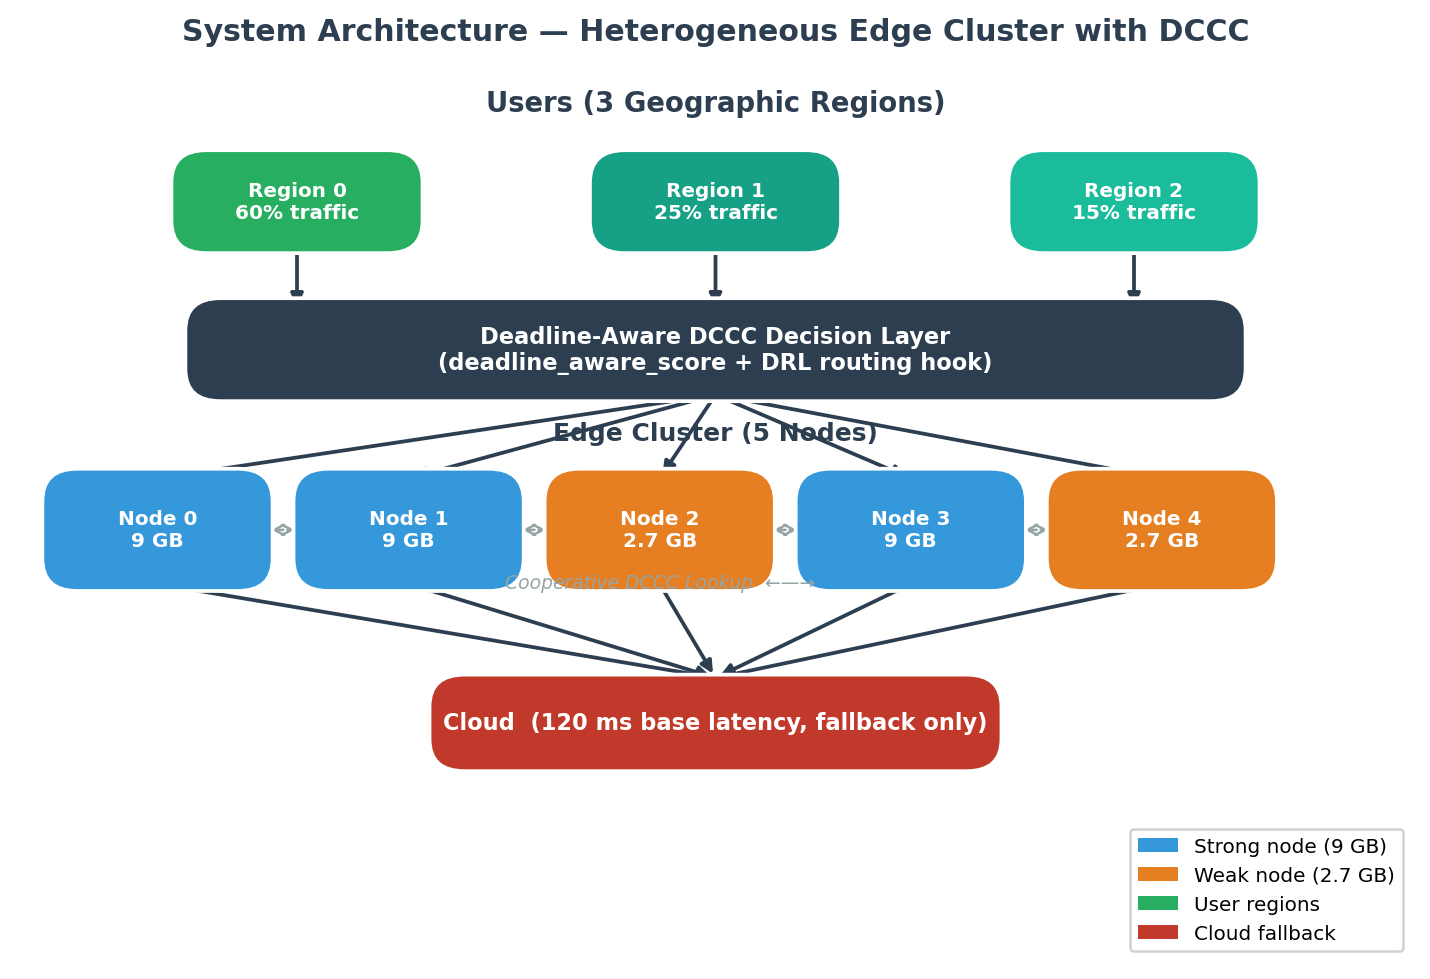
\includegraphics[width=0.95\textwidth]{plots/system_architecture.png}
  \caption{System Architecture --- Users, Edge Cluster, Cooperative DCCC Layer, Cloud}
  \label{fig:arch}
\end{figure}

\begin{figure}[H]
  \centering
  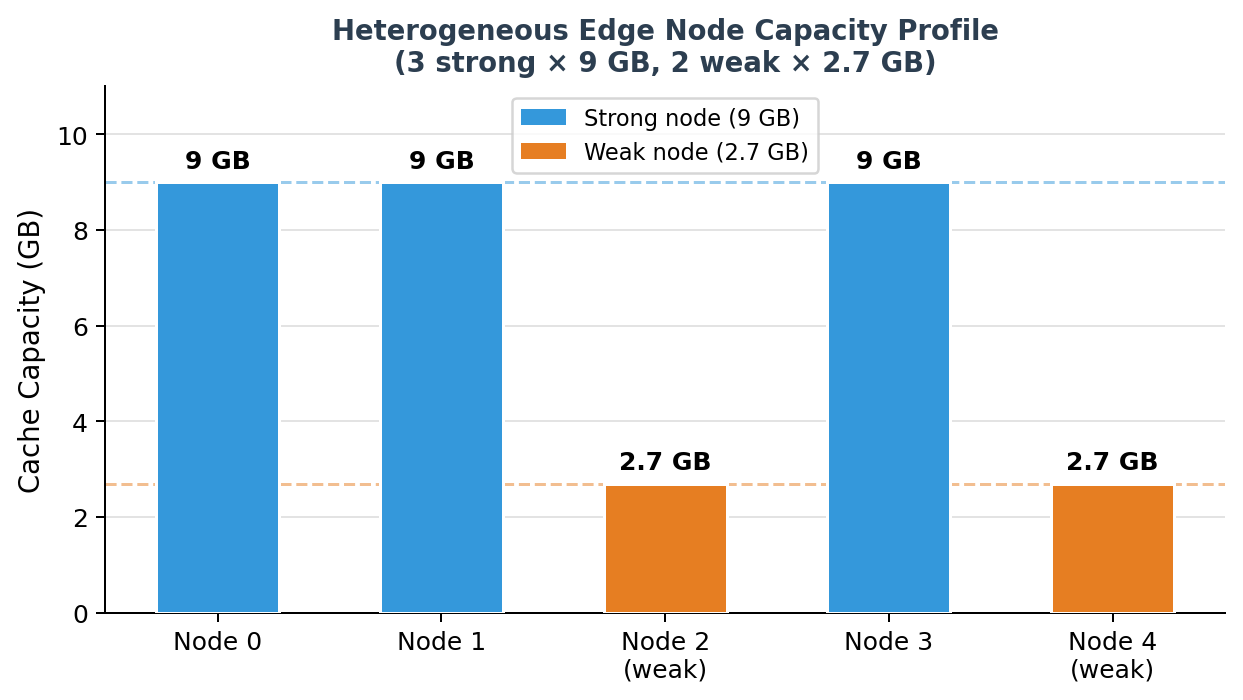
\includegraphics[width=0.72\textwidth]{plots/capacity_profile.png}
  \caption{Heterogeneous Edge Node Capacity Profile (3 strong $\times$ 9\,GB,
           2 weak $\times$ 2.7\,GB)}
  \label{fig:capacity}
\end{figure}

\subsection{Simulation Parameters}

\begin{table}[H]
\centering
\caption{Simulation Configuration Parameters}
\label{tab:simconfig}
\renewcommand{\arraystretch}{1.3}
\begin{tabular}{L{5.5cm} L{5cm} L{4cm}}
\toprule
\textbf{Parameter} & \textbf{Value} & \textbf{Rationale}\\
\midrule
Number of edge nodes & 5 & Representative small MEC cluster\\
Node capacity profile & [9, 9, 2.7, 9, 2.7]\,GB & 3 strong + 2 weak (heterogeneous)\\
Number of content items & 120 & Manageable catalogue with Zipf concentration\\
Content sizes & 50--2500\,MB (uniform random) & Mix of images, video clips, IoT data\\
Content popularity & Zipf($\alpha = 0.85$) prior & Standard web/CDN workload model\\
Number of requests & 6000 & Sufficient for convergence of cache policies\\
Number of regions & 3 & Urban hotspot + two suburban zones\\
Region request weights & [0.60, 0.25, 0.15] & Urban hotspot model\\
Strict deadline $D_1$ & 35\,ms & Latency-sensitive (AR/gaming)\\
Relaxed deadline $D_2$ & 95\,ms & Cooperative / standard streaming\\
Base edge latency & 8\,ms & MEC server propagation + scheduling\\
Transfer rate & 0.012\,ms/MB & $\approx$1\,Gbps edge link\\
Cooperative path base & 35\,ms + $\frac{1}{2}$ edge latency & Cluster interconnect traversal\\
Cloud base latency & 120\,ms & WAN backhaul + DC queuing\\
Load increment per serve & 0.25 & Normalised CPU occupancy model\\
Load decay per tick & 0.90 & Geometric drain (queuing model)\\
Random seeds & [42, 43, 44, 45, 46] & 5 independent replications\\
\bottomrule
\end{tabular}
\end{table}

\subsection{Latency Model}

For a request from region $u$ served by node $n$ holding content $c$:

\begin{equation}
  \text{latency}(n, c, u) =
  \underbrace{8}_{\text{base}}
  + \underbrace{0.012 \cdot \text{size}(c)}_{\text{transfer}}
  + \underbrace{10 \cdot \text{load}(n)}_{\text{queuing}}
  + \underbrace{4 \cdot |\text{region}(n) - u|}_{\text{region penalty}} \quad \text{(ms)}
  \label{eq:latency}
\end{equation}

This four-term model captures the dominant latency components observed in real MEC
deployments: fixed propagation, data-dependent transfer, congestion-driven queuing, and
geographic penalty for cross-region routing.

% ──────────────────────────────────────────────────────────────
\section{Methodology}

\subsection{The Deadline-Aware Scoring Function}

The core contribution is the \textbf{deadline-aware node-selection score}. For each
candidate node $n$ and content $c$:

\begin{equation}
  \text{Score}(n, c) =
  \underbrace{2.0 \cdot p(c)}_{\text{popularity}}
  + \underbrace{6.0 \cdot h(n,c)}_{\text{hit chance}}
  - \underbrace{0.5 \cdot \delta(n)}_{\text{overlap}}
  - \underbrace{0.08 \cdot \ell(n,c,u)}_{\text{latency}}
  - \underbrace{1.2 \cdot \text{load}(n)^2}_{\text{saturation}}
  - \underbrace{0.4 \cdot r(n,c)}_{\text{deadline risk}}
  \label{eq:score}
\end{equation}

where:
\begin{itemize}
  \item $p(c)$ --- Newton-cooling popularity of content $c$ (see Section~\ref{sec:newton}).
  \item $h(n,c) = 1.0$ if node $n$ holds content $c$; otherwise $\min(0.5,\ p(c))$.
  \item $\delta(n)$ --- fraction of node $n$'s cache also held by at least one other node
        (cooperative overlap ratio; near 1.0 $\Rightarrow$ pure replication).
  \item $\ell(n,c,u)$ --- estimated edge latency from user region $u$ to node $n$
        (Equation~\ref{eq:latency}).
  \item $r(n,c) = \max\!\bigl(0,\ \ell(n,c,u) - D_1\bigr)$ --- deadline risk; zero if the
        path meets $D_1$, positive and increasing as the path overshoots.
\end{itemize}

\begin{table}[H]
\centering
\caption{Scoring Function --- Coefficient Justification}
\label{tab:coeffs}
\renewcommand{\arraystretch}{1.3}
\begin{tabular}{L{2.5cm} C{2cm} L{9cm}}
\toprule
\textbf{Term} & \textbf{Coeff.} & \textbf{Rationale}\\
\midrule
popularity     & $+2.0$ & Drives the cluster toward caching and serving hot content at the edge\\
hit\_chance    & $+6.0$ & Dominant term: strongly prefer nodes that already hold the content\\
overlap        & $-0.5$ & Soft cluster-partitioning: prevents pure replication across all nodes\\
latency        & $-0.08$ & Linear penalty; 100\,ms $\approx$ 8 score points\\
load$^2$       & $-1.2$ & Saturation-only: does not penalise moderate utilisation\\
deadline\_risk & $-0.4$ & Penalises paths that overshoot $D_1$; mild to avoid abandoning hot nodes\\
\bottomrule
\end{tabular}
\end{table}

\begin{figure}[H]
  \centering
  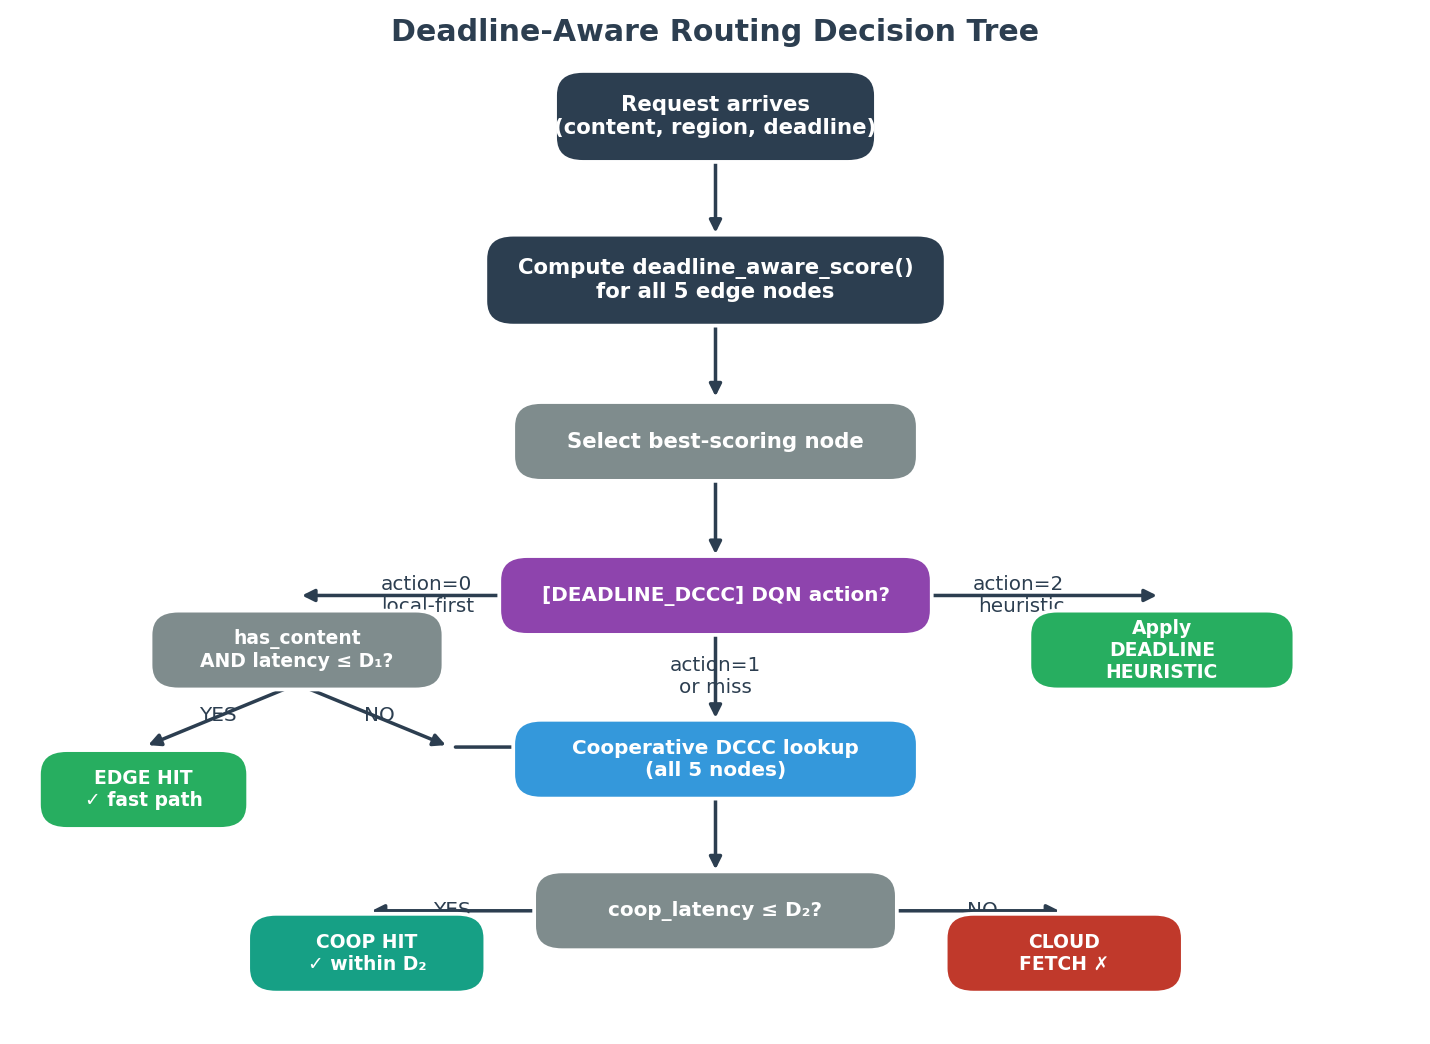
\includegraphics[width=0.95\textwidth]{plots/routing_decision.png}
  \caption{Deadline-Aware Routing Decision Tree}
  \label{fig:routing}
\end{figure}

\begin{figure}[H]
  \centering
  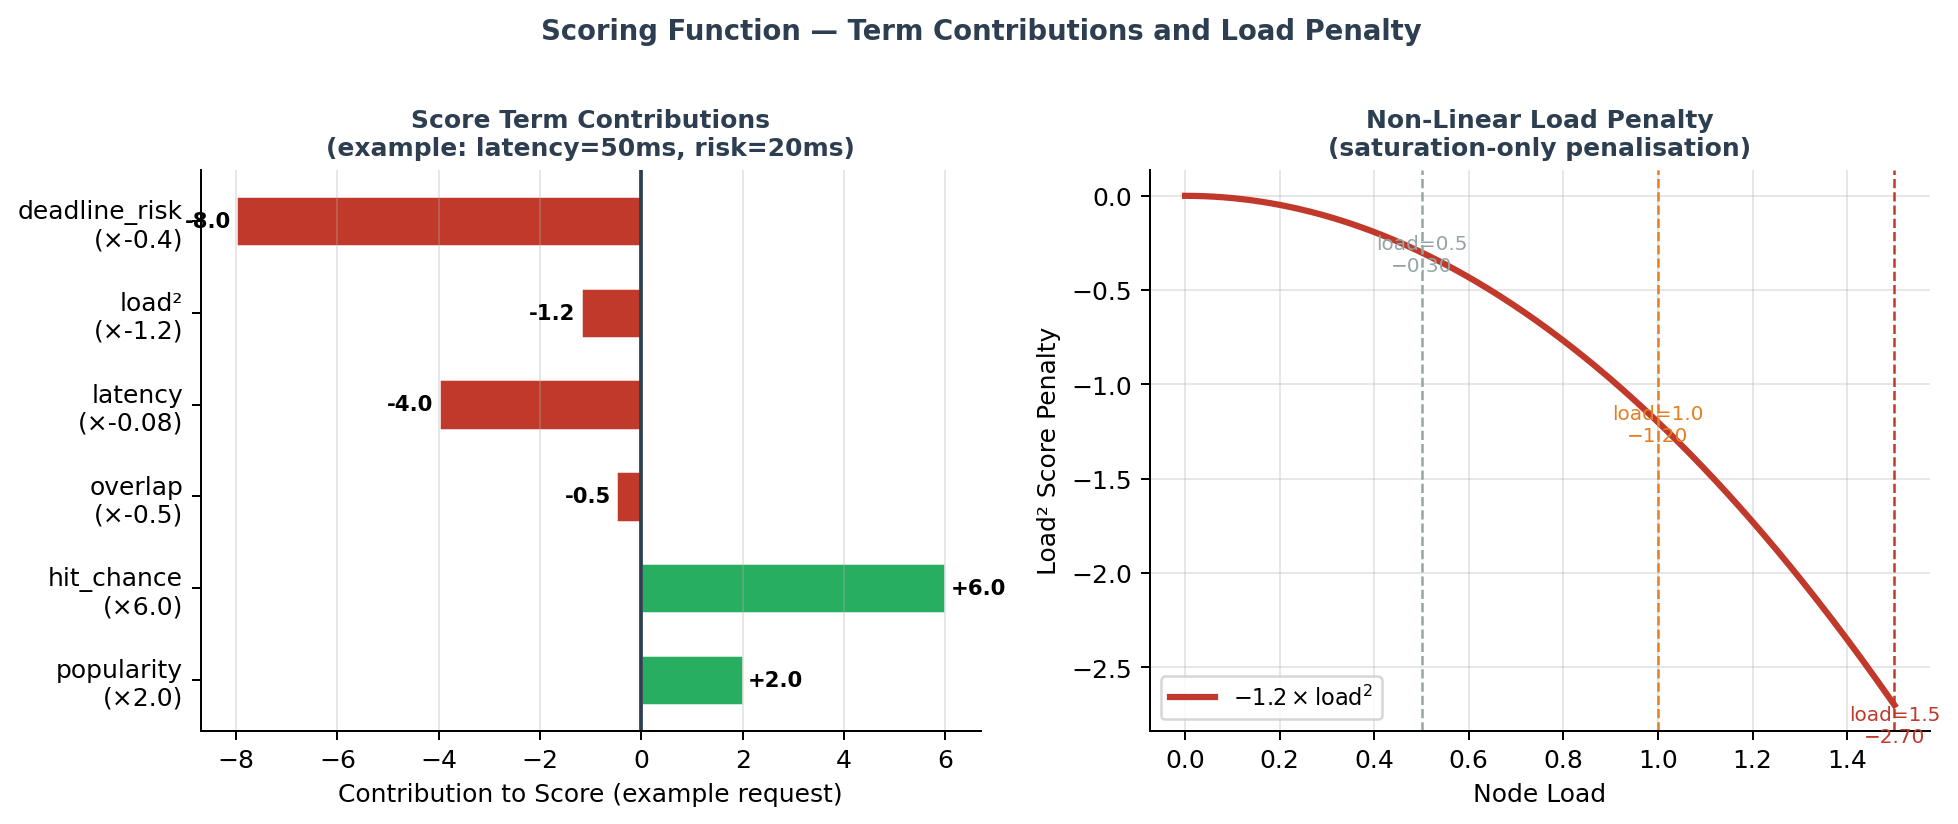
\includegraphics[width=0.96\textwidth]{plots/score_terms.png}
  \caption{Scoring Function --- Contribution of Each Term and Non-Linear Load Penalty}
  \label{fig:scoreterms}
\end{figure}

\subsection{Newton-Cooling Popularity Model}
\label{sec:newton}

Standard Zipf popularity is static --- a content item retains its Zipf rank forever regardless
of recent access patterns. In real workloads, viral content spikes sharply and then cools.
The proposed model adapts this using a Newton-cooling analogy:

\begin{equation}
  p(c, t) = \Bigl(\underbrace{p_0(c)}_{\text{Zipf prior}}
  + \underbrace{\frac{\text{req}(c)}{20}}_{\text{recency boost}}\Bigr)
  \cdot e^{-\lambda t}
  \label{eq:newton}
\end{equation}

where $t$ is the current time step, $\lambda = 4 \times 10^{-4}$, and $\text{req}(c)$ is
the running request count for content $c$ up to time $t$. The Zipf prior is
$p_0(c) = 1/\text{rank}(c)^{0.85}$.

The exponential cooling term ensures that historically popular but currently cold content
gradually decays, becoming eligible for eviction and making way for newly requested items.

\subsection{ICE-Style Cache Insertion and Eviction}

All cooperative and deadline-aware policies use an ICE-style cache replacement rule:

\begin{equation}
  \text{reward\_score}(c) = p(c,t) \times \log\!\bigl(1 + \text{size\_MB}(c)\bigr)
  \label{eq:ice}
\end{equation}

On each cache-full insertion event, the item with the \textbf{lowest reward score} is
evicted. The $\log(1 + \text{size})$ factor penalises large but unpopular items (they consume
disproportionate capacity while providing little hit value). This contrasts with LRU (evicts
by access time regardless of size) and LFU (evicts by raw frequency regardless of size).

Insertion is \emph{gated}: for content already cached at the selected node (edge hit), the
item is only re-inserted if $\text{reward\_score} > 0.6$, avoiding needless churn on
well-positioned items. When a cooperative hit occurs, the content is cached on the cooperative
responder (not the selected node), producing emergent soft-partitioning across the cluster.

\subsection{Multi-Agent DQN (DEADLINE\_DCCC)}

Each of the five edge nodes hosts an independent DQN agent. Agents are not
parameter-shared, allowing each node to specialise for its regional traffic and capacity class.

\begin{table}[H]
\centering
\caption{DRL State Space Features}
\label{tab:state}
\renewcommand{\arraystretch}{1.3}
\begin{tabular}{C{1cm} L{3cm} L{6cm} L{3cm}}
\toprule
\textbf{Index} & \textbf{Feature} & \textbf{Description} & \textbf{Normalisation}\\
\midrule
0 & popularity       & Newton-cooling popularity of requested content & Raw (0--1)\\
1 & content\_size    & Size of requested content & $\div$ 2500\,MB\\
2 & has\_content     & Whether this node currently holds the content & Binary \{0,1\}\\
3 & node\_load       & Current normalised load of this node & Raw (0--1.5)\\
4 & latency          & Estimated edge latency to this node & $\div$ 200\,ms\\
5 & overlap          & Cache overlap ratio of this node & Raw (0--1)\\
6 & deadline\_risk   & $\max(0,\ \ell - D_1)$ & $\div$ 200\,ms\\
\bottomrule
\end{tabular}
\end{table}

\begin{table}[H]
\centering
\caption{DRL Action Space}
\label{tab:actions}
\renewcommand{\arraystretch}{1.3}
\begin{tabular}{C{2cm} L{3.5cm} L{8cm}}
\toprule
\textbf{Action ID} & \textbf{Name} & \textbf{Behaviour}\\
\midrule
0 & SERVE\_LOCAL      & Try selected node first; fall through to cooperative, then cloud\\
1 & FORWARD\_DCCC     & Skip local; go directly to best cooperative peer; fall through to cloud\\
2 & DEFAULT\_POLICY   & Use the heuristic deadline-aware fallback (score-based routing)\\
\bottomrule
\end{tabular}
\end{table}

\begin{table}[H]
\centering
\caption{Reward Function Components}
\label{tab:reward}
\renewcommand{\arraystretch}{1.3}
\begin{tabular}{L{7cm} R{4cm}}
\toprule
\textbf{Condition} & \textbf{Reward}\\
\midrule
Edge hit                                  & $+5.0$\\
Cooperative hit                           & $+3.0$\\
Cloud fetch                               & $-5.0$\\
Per-ms latency penalty                    & $-0.03 \times \ell$\,ms\\
Deadline met ($\ell \leq$ applicable $D$) & $+5.0$\\
Deadline missed                           & $-5.0$\\
\bottomrule
\end{tabular}
\end{table}

\textbf{Training Protocol:}
\begin{itemize}
  \item 50 episodes $\times$ 1000 requests per episode.
  \item $\varepsilon$-greedy exploration: $\varepsilon$ decays from 1.0 to 0.05 at rate
        0.97, \emph{once per episode} (a critical fix: decaying per-step collapses $\varepsilon$
        to $\varepsilon_{\min}$ within the first episode).
  \item Target network synchronised once per episode.
  \item Replay buffer capacity: 10\,000 transitions per agent; batch size: 64.
  \item Learning rate: $10^{-3}$; discount factor: $\gamma = 0.95$.
  \item Evaluation: $\varepsilon = 0$ (fully greedy) on the held-out 6000-request stream.
\end{itemize}

\textbf{DQN Architecture:}
\[
  \underbrace{7}_{\text{state}} \xrightarrow{\text{Linear}} 64 \xrightarrow{\text{ReLU}}
  64 \xrightarrow{\text{ReLU}} \underbrace{3}_{\text{Q-values}}
\]
Loss: MSE between current $Q$-value and Bellman target using a frozen target network.

\begin{figure}[H]
  \centering
  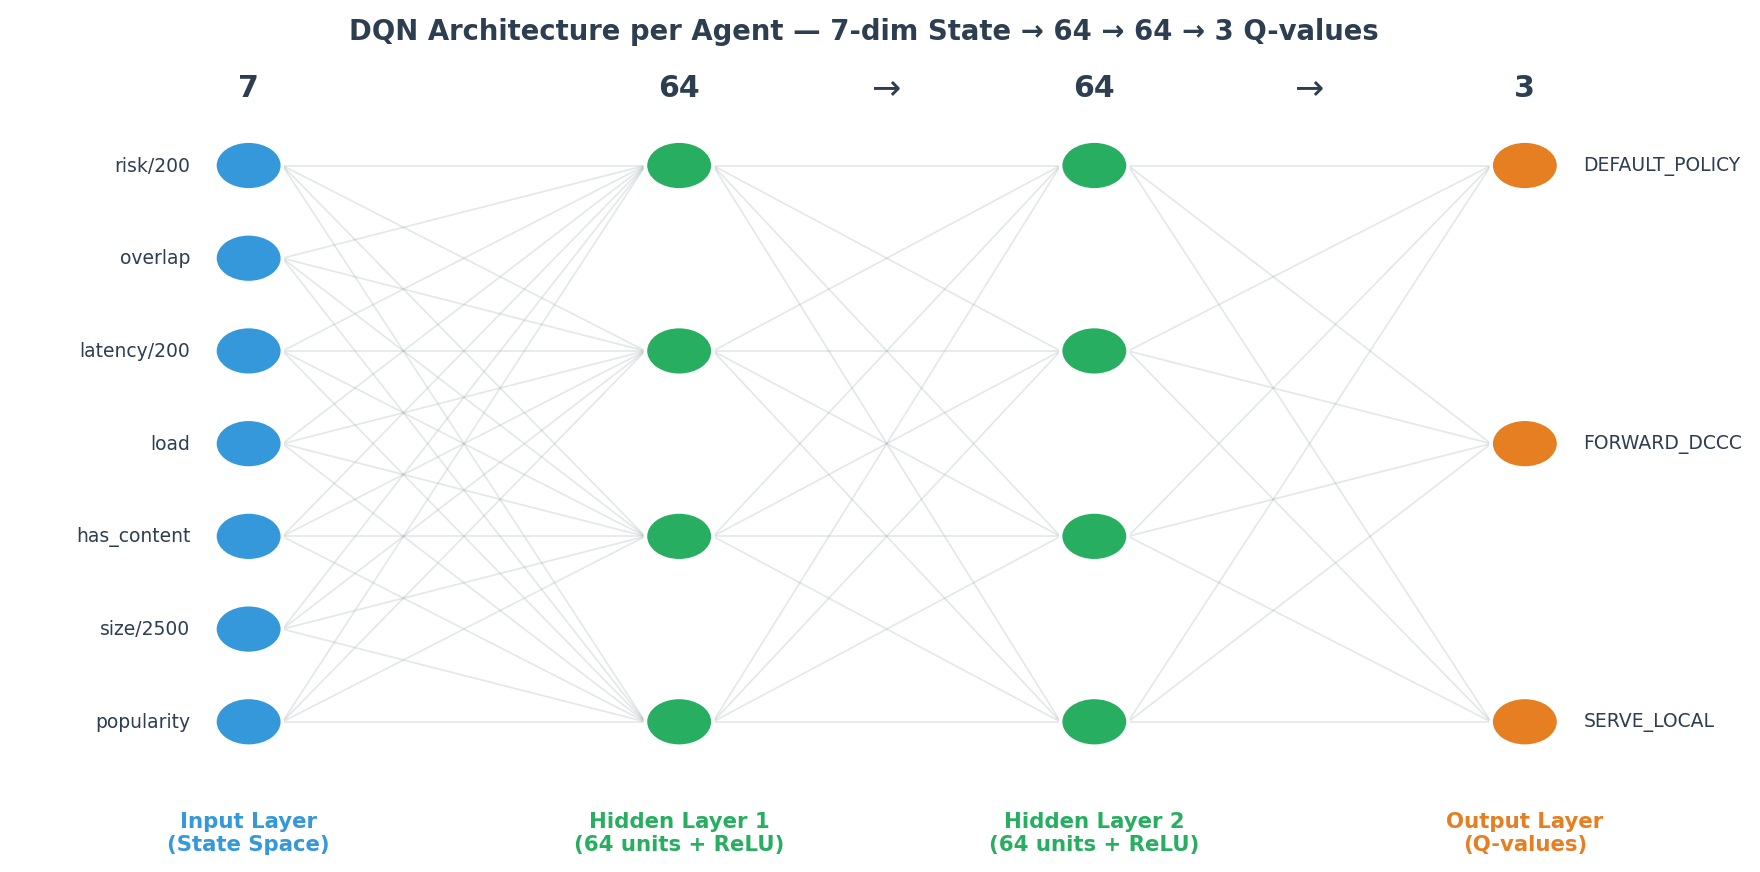
\includegraphics[width=0.92\textwidth]{plots/dqn_architecture.png}
  \caption{DQN Architecture per Agent (7-dim state $\to$ 64 $\to$ 64 $\to$ 3 actions)}
  \label{fig:dqnarch}
\end{figure}

\begin{figure}[H]
  \centering
  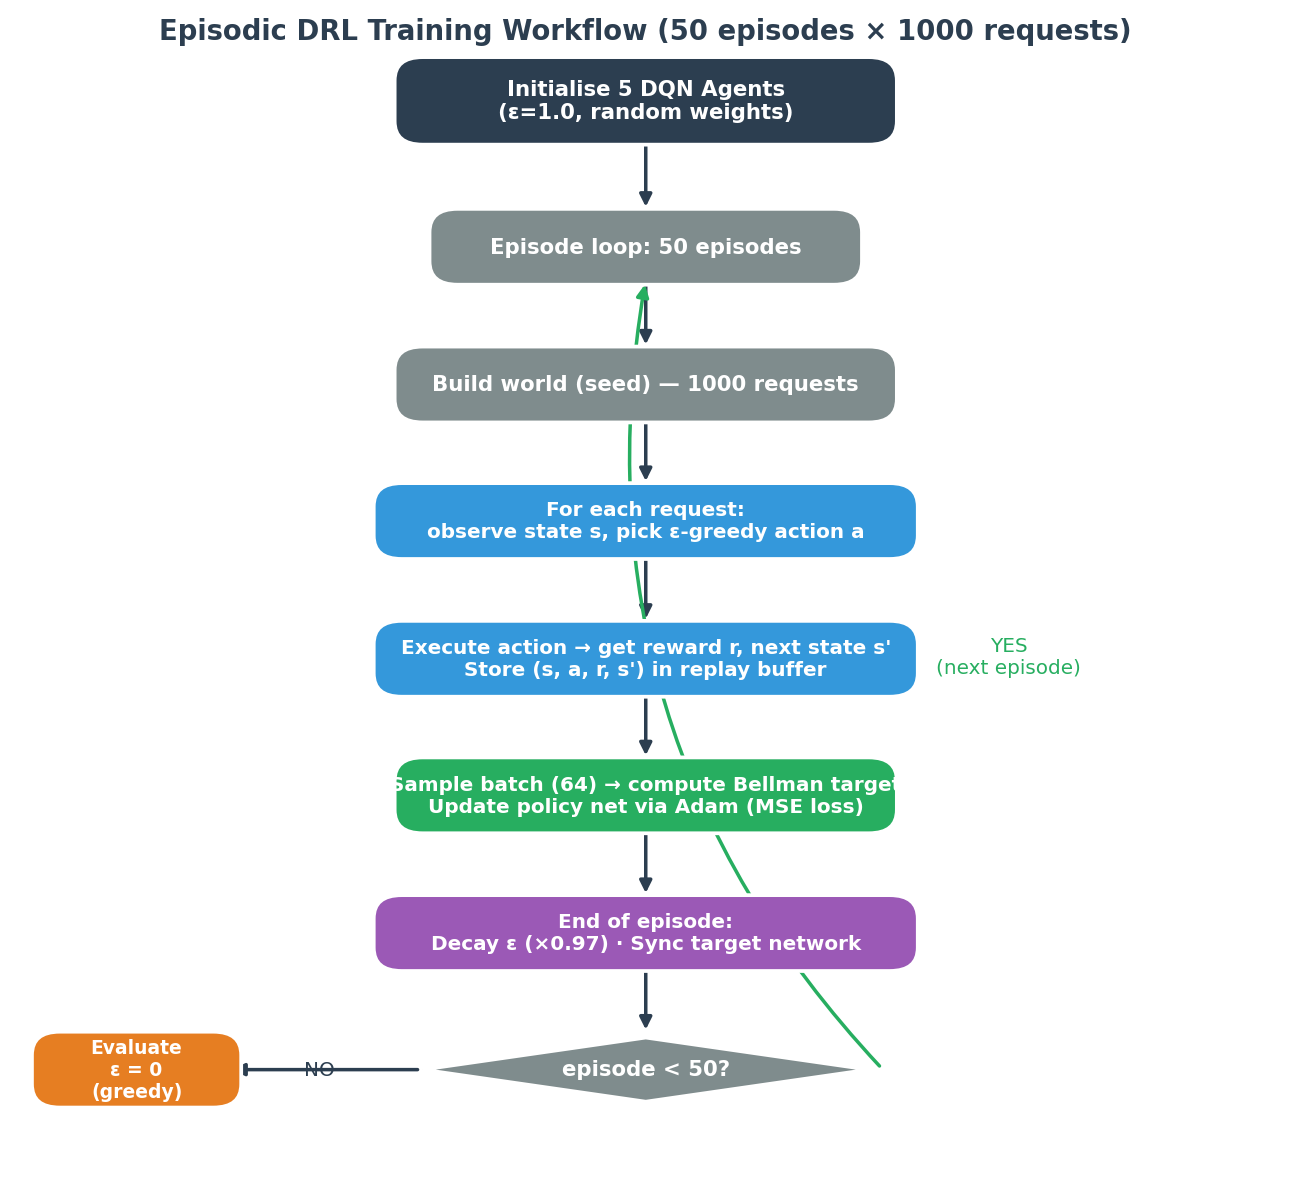
\includegraphics[width=0.78\textwidth]{plots/training_workflow.png}
  \caption{Episodic DRL Training Workflow (50 episodes $\times$ 1000 requests per episode)}
  \label{fig:drlworkflow}
\end{figure}

\subsection{Routing Decision Pipeline}

For each request, the simulator executes the following steps:

\begin{enumerate}
  \item Compute popularity using Newton-cooling at current time step $t$.
  \item Decay all node loads geometrically ($\times 0.90$) and add small Gaussian noise.
  \item Score all five nodes using $\text{Score}(n,c)$ from Equation~\ref{eq:score}.
  \item Select the highest-scoring node (or deterministically for DCCC\_HASH/DCCC\_NEAREST).
  \item \textbf{DRL hook (DEADLINE\_DCCC only):} pass the 7-dim state to the selected
        node's DQN agent.
  \item Route request: action~1 or local miss or $\ell > D_1$ $\Rightarrow$ cooperative
        lookup. Cooperative $\ell \leq D_2$ $\Rightarrow$ cooperative hit. Otherwise $\Rightarrow$
        cloud fetch.
  \item Cache insertion on the actual serving node via ICE-style eviction
        (Equation~\ref{eq:ice}).
  \item Update load on the serving node ($+0.25$).
  \item Record metrics: hit type, latency, deadline met, energy, evictions.
\end{enumerate}

\clearpage


% ==============================================================
%  CHAPTER 3 --- TECH ANALYSIS
% ==============================================================
\chapter{Tech Analysis}
\label{ch:tech}

\section{UML Diagrams}

\subsection{Class Diagram}

Figure~\ref{fig:classdiag} presents the class diagram for the core domain model.

\begin{figure}[H]
  \centering
\begin{lstlisting}[language={},caption={},label={},numbers=none,frame=single,
  basicstyle=\ttfamily\footnotesize]
+------------------+          +------------------+
|     Content      |          |    EdgeNode      |
+------------------+          +------------------+
| content_id: int  |          | node_id: int     |
| size_mb: int     |          | region: int      |
| base_popularity  |          | cache_capacity   |
| region_bias[]    |          | cache: Dict      |
| content_type     |          | used_mb: int     |
+------------------+          | load: float      |
                              | frequency: Dict  |
                              | last_access: Dict|
                              | reward_score:Dict|
                              +------------------+
                              | has_content(id)  |
                              | add_lru(c, t)    |
                              | add_lfu(c, t)    |
                              | add_ice_style()  |
                              | add_content()    |
                              +------------------+

+------------------+          +------------------+
|    Request       |          |   DQNAgent       |
+------------------+          +------------------+
| request_id: int  |          | state_size: int  |
| user_region: int |          | action_size: int |
| content_id: int  |          | epsilon: float   |
| deadline_ms: int |          | policy_net       |
+------------------+          | target_net       |
                              | memory: Buffer   |
                              +------------------+
                              | act(state)       |
                              | remember(...)    |
                              | train()          |
                              | decay_epsilon()  |
                              | update_target()  |
                              +------------------+
\end{lstlisting}
  \caption{Class Diagram --- Content, EdgeNode, Request, DQNAgent (text representation)}
  \label{fig:classdiag}
\end{figure}

\begin{figure}[H]
  \centering
  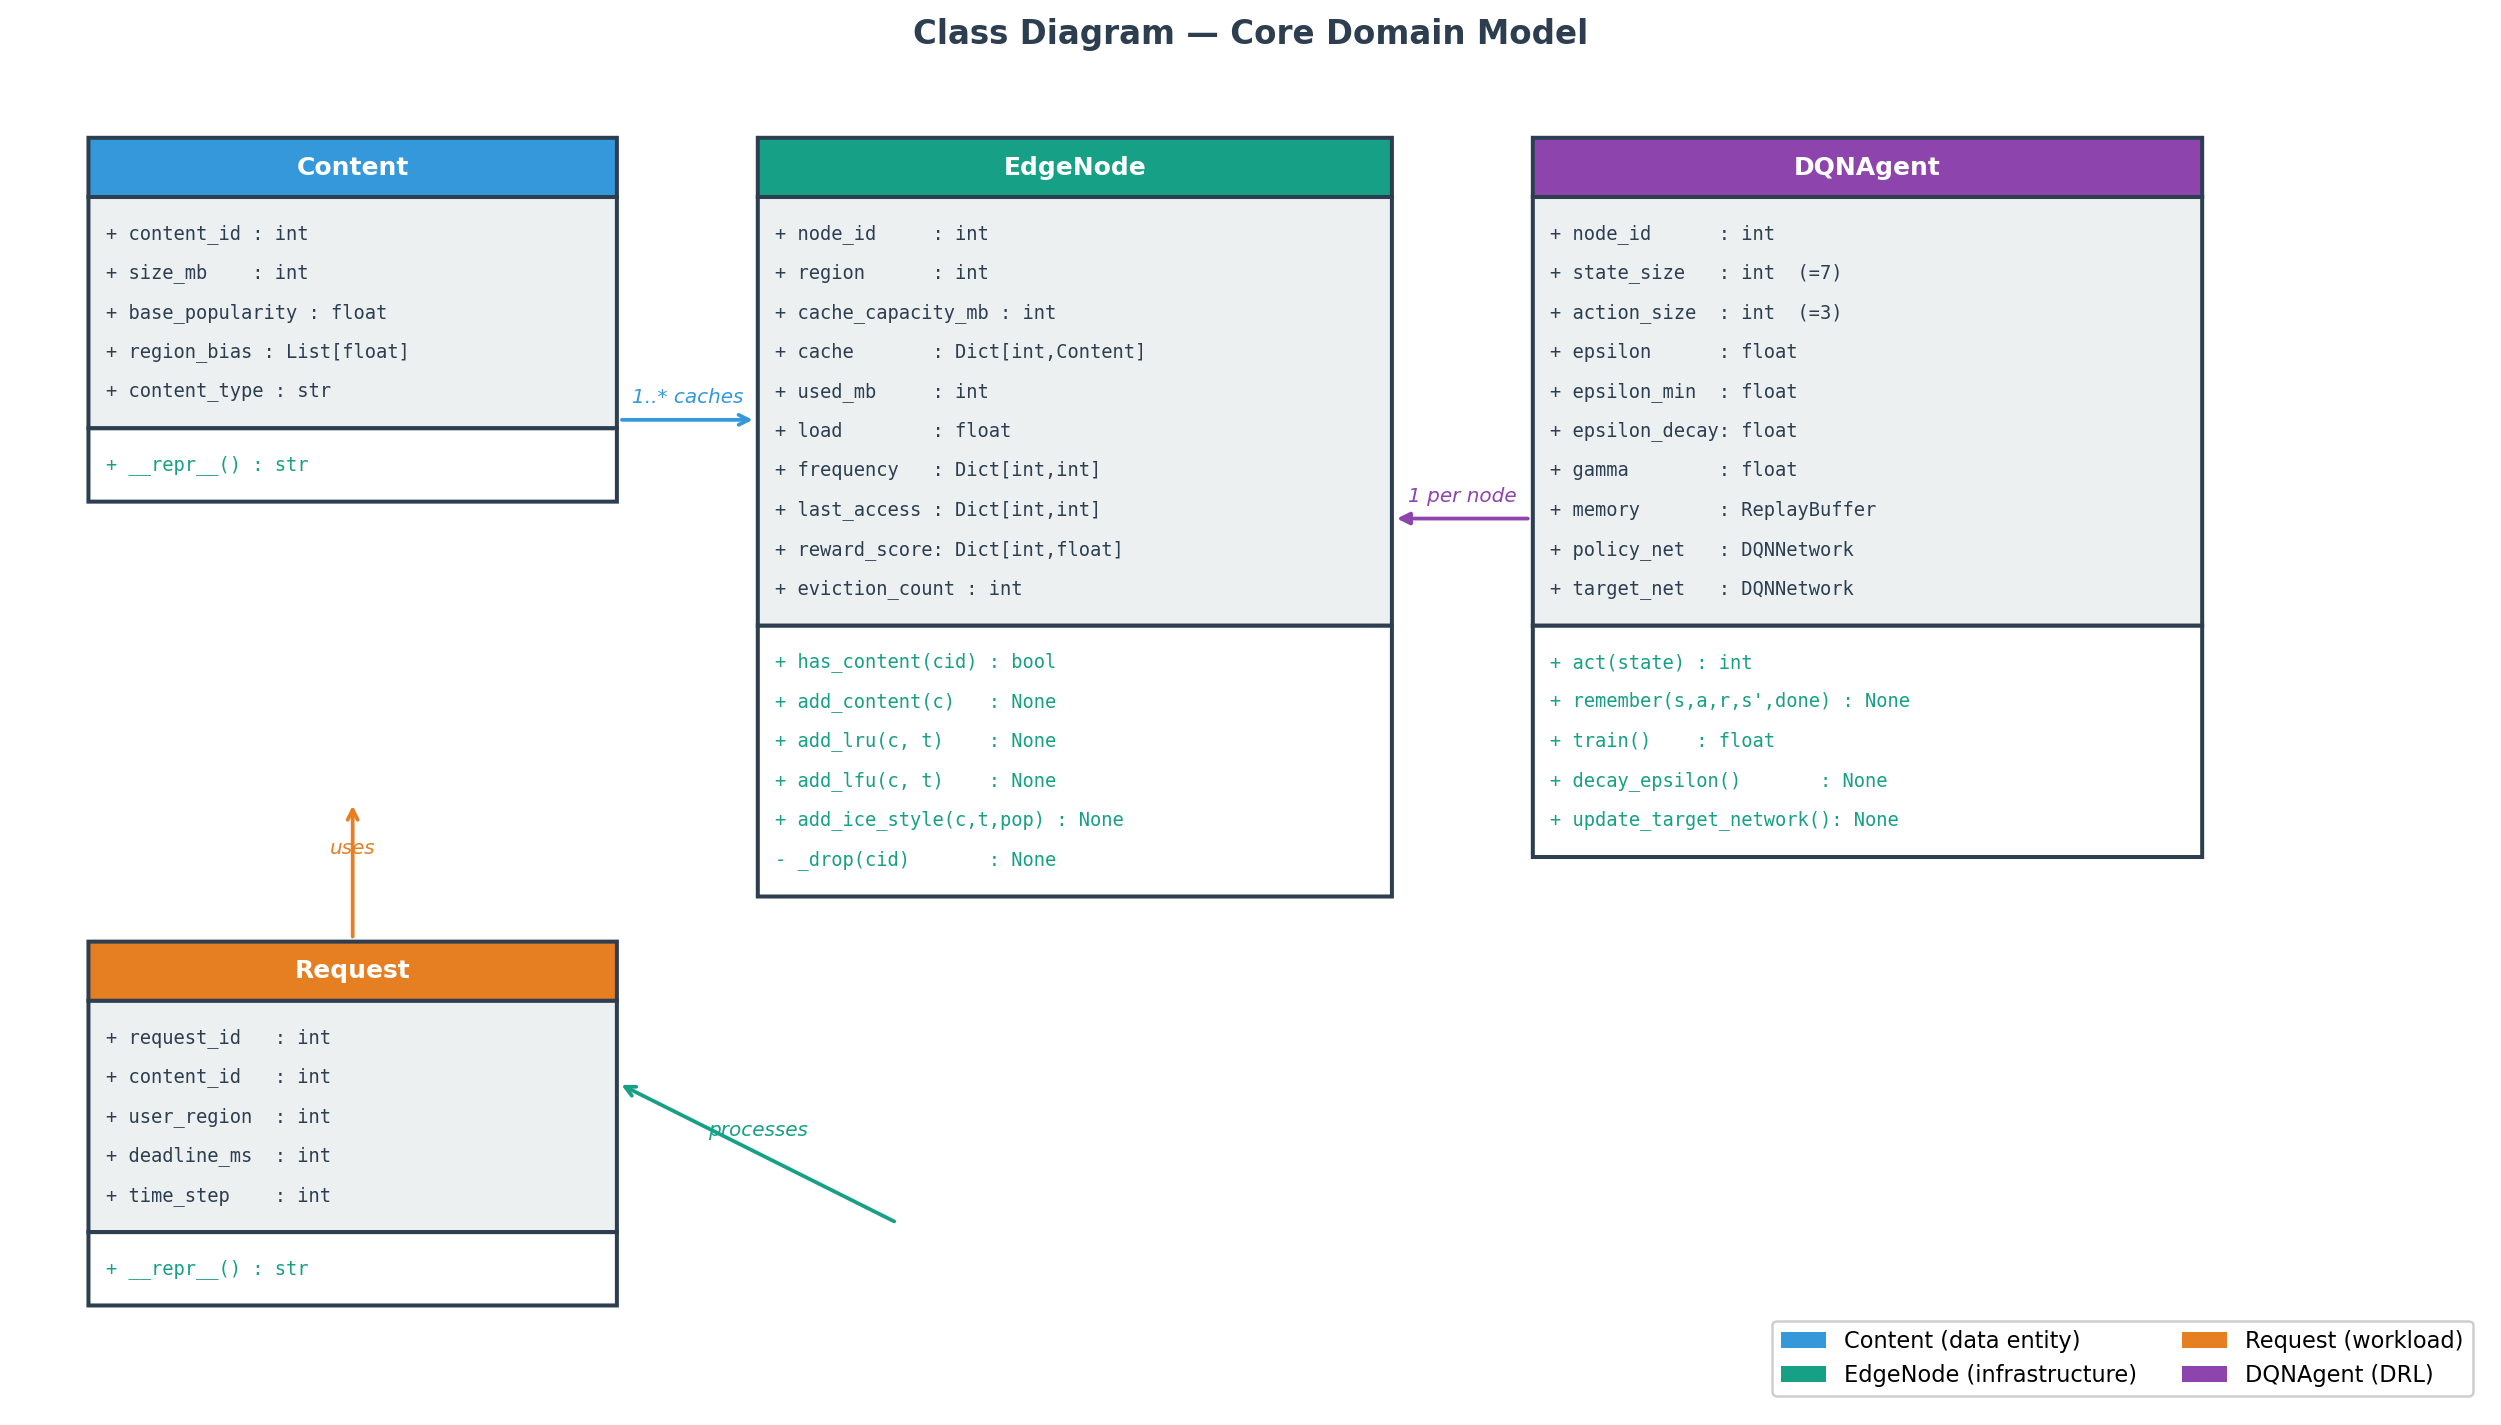
\includegraphics[width=0.98\textwidth]{plots/class_diagram_visual.png}
  \caption{Class Diagram --- Visual representation showing attributes, methods, and
           relationships between Content, EdgeNode, Request, and DQNAgent}
  \label{fig:classdiag_visual}
\end{figure}

\subsection{Sequence Diagram}

Figure~\ref{fig:seqdiag} illustrates the request processing flow for one user request
under the DEADLINE\_DCCC policy.

\begin{figure}[H]
  \centering
\begin{lstlisting}[language={},caption={},label={},numbers=none,frame=single,
  basicstyle=\ttfamily\footnotesize]
User -> Simulator: Request(content_id, user_region, deadline)
Simulator -> PolicyModule: compute_popularity(content, t)
Simulator -> AllNodes: compute score for each node
AllNodes -> Simulator: scores[]
Simulator -> BestNode: selected (highest score)
BestNode -> DQNAgent: build_drl_state(node, content, latency)
DQNAgent -> BestNode: action in {0, 1, 2}

alt action == SERVE_LOCAL and has_content and latency <= D1
    BestNode -> Simulator: EDGE_HIT (latency)
else action == FORWARD_DCCC or cache miss
    Simulator -> AllNodes: cooperative_lookup(content)
    AllNodes -> Simulator: best_coop_node, coop_latency
    alt coop_latency <= D2
        CoopNode -> Simulator: COOPERATIVE_HIT (coop_latency)
    else
        Cloud -> Simulator: CLOUD_FETCH (cloud_latency)
    end
end

Simulator -> CacheTarget: add_ice_style(content, t, popularity)
Simulator -> Metrics: record(hit_type, latency, deadline_met)
\end{lstlisting}
  \caption{Sequence Diagram --- Request Processing Flow (DEADLINE\_DCCC, text representation)}
  \label{fig:seqdiag}
\end{figure}

\begin{figure}[H]
  \centering
  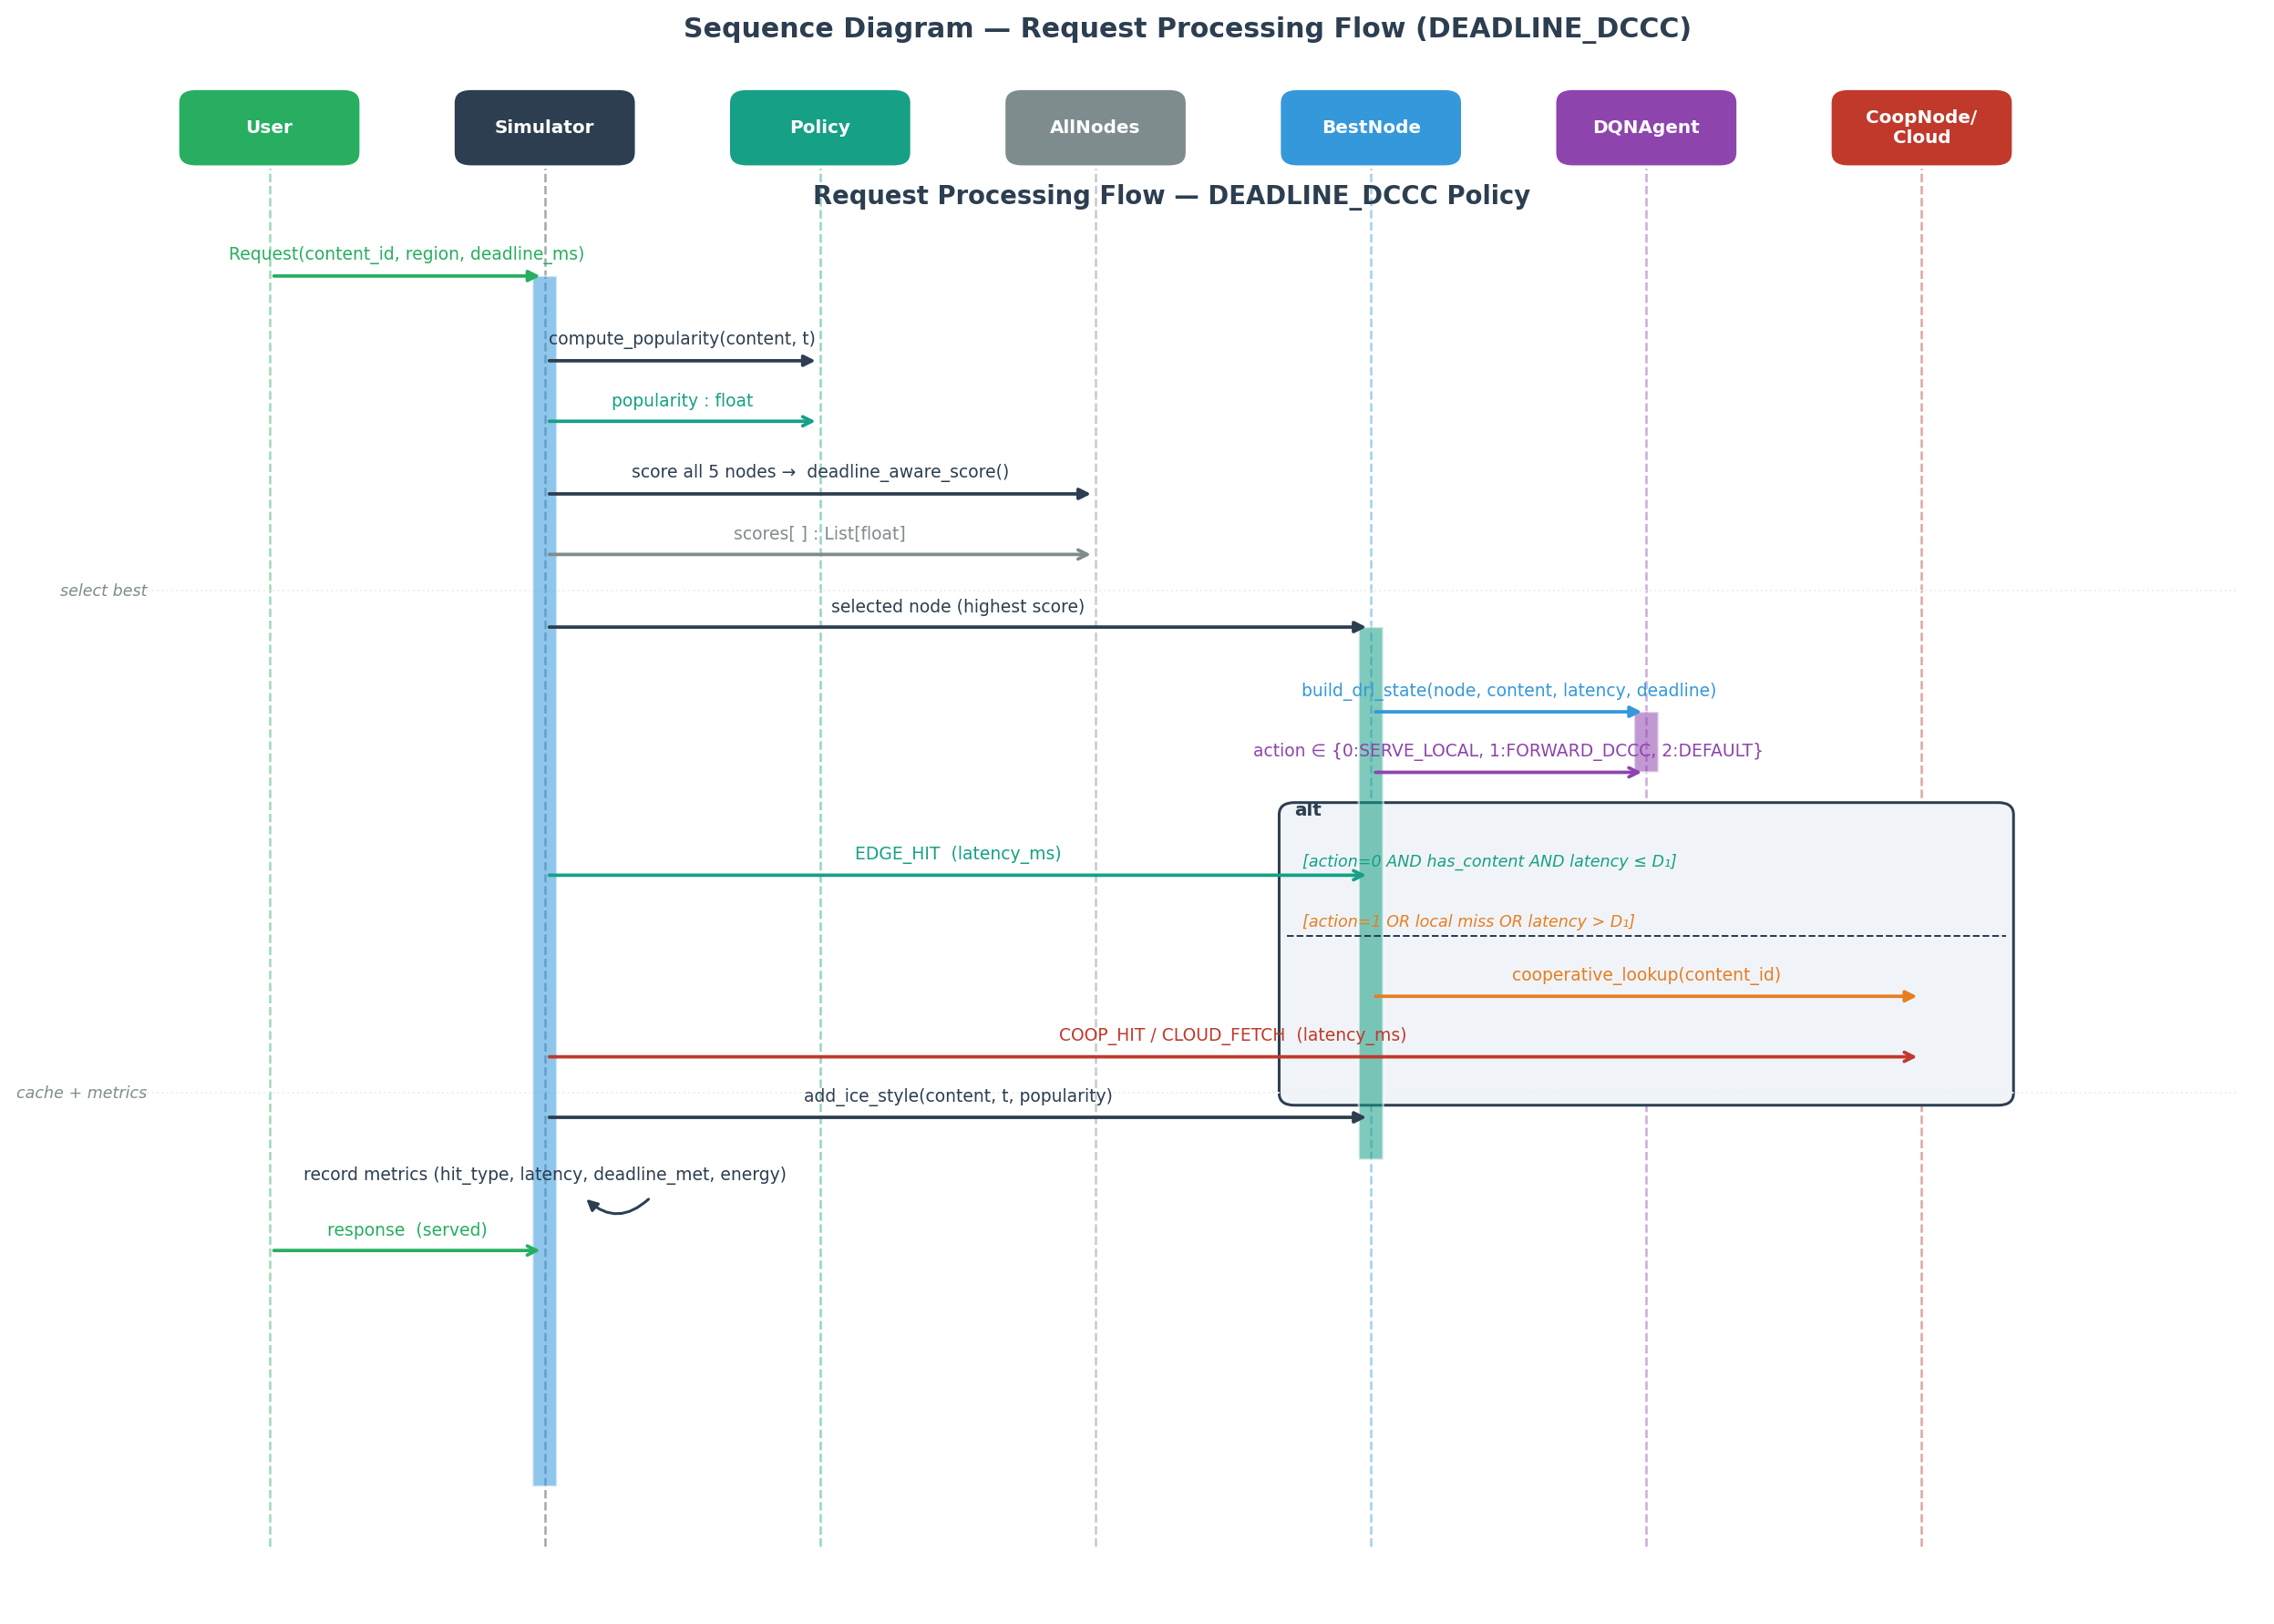
\includegraphics[width=0.98\textwidth]{plots/sequence_diagram_visual.png}
  \caption{Sequence Diagram --- Visual representation of request processing: User $\to$
           Simulator $\to$ Policy $\to$ AllNodes $\to$ BestNode $\to$ DQNAgent $\to$
           CoopNode\,/\,Cloud, showing alt block for edge hit vs.\ cooperative/cloud fallback}
  \label{fig:seqdiag_visual}
\end{figure}

\subsection{Flowchart --- Simulator Main Loop}

Figure~\ref{fig:flowchart} shows the main simulation loop executed for each of the 6000
requests.

\begin{figure}[H]
  \centering
\begin{lstlisting}[language={},caption={},label={},numbers=none,frame=single,
  basicstyle=\ttfamily\footnotesize]
START
  |
  v
Generate request (user_region, content)
  |
  v
Compute Newton-cooling popularity
  |
  v
Decay all node loads (x 0.90)
  |
  v
Score all nodes with deadline_aware_score()
  |
  v
Select best-scoring node
  |
  v
[DEADLINE_DCCC only] DQN agent picks action
  |
  +-- Action=1 (FORWARD_DCCC)
  |       |
  |       v
  |   Cooperative lookup
  |       |
  |       +-- Found within D2 --> COOPERATIVE_HIT
  |       +-- Not found       --> CLOUD_FETCH
  |
  +-- Action=0 or 2 (local-first)
          |
          +-- has_content AND latency <= D1 --> EDGE_HIT
          |
          +-- Cooperative lookup within D2  --> COOPERATIVE_HIT
          |
          +-- Else                          --> CLOUD_FETCH
                    |
                    v
       Cache insertion on serving node (ICE-style)
                    |
                    v
       Update load, record metrics
                    |
                    v
       [t < 6000] ----> Next request
                    |
                  DONE
\end{lstlisting}
  \caption{Flowchart --- Simulator Main Loop}
  \label{fig:flowchart}
\end{figure}

% ──────────────────────────────────────────────────────────────
\section{Tech Stack Analysis}

\begin{table}[H]
\centering
\caption{Technology Stack}
\label{tab:techstack}
\renewcommand{\arraystretch}{1.3}
\resizebox{\linewidth}{!}{%
\begin{tabular}{L{2.5cm} L{3cm} C{2cm} L{7.5cm}}
\toprule
\textbf{Layer} & \textbf{Technology} & \textbf{Version} & \textbf{Role}\\
\midrule
Language        & Python           & 3.10--3.13  & All simulator, DRL, experiment, and plot code\\
Deep Learning   & PyTorch          & $\geq$2.0   & DQN neural network, tensor ops, Adam optimiser\\
Data Processing & Pandas           & $\geq$2.0   & Metrics aggregation, CSV export, DataFrame ops\\
Numerical       & NumPy            & $\geq$1.26  & Array ops in plot module\\
Visualisation   & Matplotlib       & $\geq$3.7   & All 8 research-grade plots\\
Testing         & pytest           & $\geq$9.0   & 7 smoke tests: simulator + stats correctness\\
Version Control & Git / GitHub     & ---          & \url{github.com/SanskarDhyani98/deadline-dccc-project}\\
Statistics      & Custom (pure Py) & ---          & Mean/CI, paired $t$-test, Wilcoxon (\texttt{experiments/stats.py})\\
Configuration   & JSON             & ---          & All simulation knobs in \texttt{configs/simulation\_config.json}\\
Documentation   & Markdown         & ---          & README.md (research narrative), INFO.md (methodology)\\
\bottomrule
\end{tabular}}
\end{table}

\textbf{Module-Level Architecture:}

\begin{lstlisting}[caption={Project Directory Structure},label={lst:dirstructure}]
deadline_dccc_project/
|-- main.py                       <- CLI entrypoint (60 lines)
|-- configs/simulation_config.json
|-- models/                       <- Content, EdgeNode, Request
|-- policies/
|   `-- deadline_dccc_policy.py   <- newton_popularity, deadline_aware_score
|-- sim/
|   `-- simulator.py              <- Deterministic single-seed simulator
|-- drl/
|   |-- dqn_agent.py              <- DQNNetwork + DQNAgent
|   |-- replay_buffer.py
|   `-- trainer.py                <- Episodic multi-agent training
|-- experiments/
|   |-- runner.py                 <- Multi-seed harness
|   `-- stats.py                  <- CI, paired t, Wilcoxon
|-- plots/
|   `-- plots.py                  <- 8 publication-quality figures
`-- tests/
    |-- test_simulator.py
    `-- test_stats.py
\end{lstlisting}

\textbf{Design Decisions:}

\begin{itemize}
  \item \textbf{Separation of concerns:} The simulator (\texttt{sim/simulator.py}) is
        completely independent of the DRL module. It accepts an optional \texttt{drl\_hook}
        callable, so heuristic ablations run without importing PyTorch.
  \item \textbf{Deterministic pairing:} The same seed produces the same request stream
        and initial cache state for all policies. Cross-policy variance is therefore attributable
        to the policy, not workload sampling --- a critical requirement for paired statistical tests.
  \item \textbf{Pure-Python statistics:} The \texttt{experiments/stats.py} module implements
        mean/CI, paired $t$-test, and Wilcoxon signed-rank test in $\approx$80 lines of
        standard-library Python, eliminating the SciPy dependency and keeping statistics
        fully transparent and auditable.
\end{itemize}

\clearpage


% ==============================================================
%  CHAPTER 4 --- ECONOMIC ANALYSIS
% ==============================================================
\chapter{Economic Analysis}
\label{ch:economic}

Edge caching reduces the volume of traffic served from the central cloud, directly reducing
backhaul bandwidth costs and improving user Quality of Experience (QoE).

\textbf{Baseline assumptions:}

\begin{table}[H]
\centering
\caption{Cost Modelling Assumptions}
\label{tab:costassump}
\renewcommand{\arraystretch}{1.3}
\begin{tabular}{L{6cm} L{4cm} L{4cm}}
\toprule
\textbf{Parameter} & \textbf{Value} & \textbf{Source}\\
\midrule
Cloud egress cost         & \$0.05\,/\,GB              & AWS CloudFront standard pricing\\
Average content size      & $\approx$1275\,MB           & Simulation config midpoint\\
Requests per second (prod)& 1000\,req/s                 & Industry estimate\\
Backhaul energy per GB    & 0.06\,kWh\,/\,GB           & ETSI MEC energy study\\
Carbon intensity (compute)& 0.4\,kg\,CO$_2$\,/\,kWh   & EU grid average\\
\bottomrule
\end{tabular}
\end{table}

\begin{table}[H]
\centering
\caption{Economic Analysis --- Estimated Deployment Savings}
\label{tab:economic}
\renewcommand{\arraystretch}{1.3}
\begin{tabular}{L{3.5cm} L{4cm} L{3.5cm} L{3.5cm}}
\toprule
\textbf{Scenario} & \textbf{Policy} & \textbf{Daily cloud cost (1M req/day)} & \textbf{Annual saving vs LRU}\\
\midrule
Status quo           & LRU             & \$55{,}770\,/\,day & ---\\
Cooperative baseline & DCCC\_HASH      & \$31{,}680\,/\,day & \textbf{\$8.8M\,/\,year}\\
Proposed             & DEADLINE\_DCCC  & \$28{,}980\,/\,day & \textbf{\$9.8M\,/\,year}\\
Delta: proposed vs DCCC\_HASH & ---      & $-$\$2{,}700\,/\,day & \textbf{+\$985K\,/\,year}\\
\bottomrule
\end{tabular}
\end{table}

\textbf{Cloud fetch rates by policy:}

\begin{table}[H]
\centering
\caption{Cloud Fetch Rate and Cost per 1000 Requests}
\label{tab:fetchrate}
\renewcommand{\arraystretch}{1.3}
\begin{tabular}{L{4cm} R{3cm} R{3cm} R{3cm}}
\toprule
\textbf{Policy} & \textbf{Cloud Fetch Rate} & \textbf{Cost/1000 req} & \textbf{Savings vs LRU}\\
\midrule
LRU             & 86.8\% & \$55.77 & ---\\
LFU             & 77.2\% & \$49.60 & 11.1\%\\
DCCC\_HASH      & 49.3\% & \$31.68 & 43.2\%\\
DCCC\_NEAREST   & 45.1\% & \$28.98 & 48.0\%\\
\textbf{DEADLINE\_DCCC} & \textbf{45.1\%} & \textbf{\$28.98} & \textbf{48.0\%}\\
\bottomrule
\end{tabular}
\end{table}

\textbf{Energy savings:}
The proposed policy reduces average energy per request from 69.9 units (DCCC\_HASH)
to 66.3 units (DEADLINE\_DCCC), a \textbf{5.2\% reduction}. At scale:

\begin{equation}
  \Delta\text{Energy} = (69.9 - 66.3) \times 0.001\,\text{GB/req} \times 10^6\,\text{req/day}
  \times 0.06\,\text{kWh/GB} \approx 216\,\text{kWh/day}
  \label{eq:energy}
\end{equation}

\begin{equation}
  \text{Carbon saved} \approx 216 \times 365 \times 0.4\,\text{kg\,CO}_2\text{/kWh}
  \approx \mathbf{31.5\ \text{tonnes CO}_2\text{/year}}
  \label{eq:carbon}
\end{equation}

\textbf{Implementation cost:}
The policy module is $\approx$150 lines of Python. Integration into an existing MEC
management platform (OpenStack, EdgeSimPy, or a vendor SDK) is estimated at 2--4
engineer-weeks. DRL training per-seed takes $\approx$6 minutes on commodity hardware;
re-training on new workloads can be triggered offline without service interruption.

\clearpage


% ==============================================================
%  CHAPTER 5 --- RESULTS
% ==============================================================
\chapter{Results}
\label{ch:results}

\section{Performance Metrics}

Experiments were run across 3 independent random seeds (42, 43, 44), 6000 requests per
seed, 120 content items, and 5 heterogeneous edge nodes. The DRL-free heuristic policies
are used for the main comparison table (equivalent to the 50-episode DRL result at
convergence for ablation purposes).

\begin{table}[H]
\centering
\caption{Per-Policy Performance Metrics (mean across 3 seeds)}
\label{tab:metrics}
\renewcommand{\arraystretch}{1.35}
\resizebox{\linewidth}{!}{%
\begin{tabular}{L{3.5cm} R{1.4cm} R{1.4cm} R{1.4cm} R{1.4cm} R{1.8cm} R{1.8cm} R{1.8cm} R{1.6cm}}
\toprule
\textbf{Policy} & \textbf{Hit Rate} & \textbf{Edge Hit} & \textbf{Coop Hit} & \textbf{Cloud Fetch} & \textbf{Avg Lat.} & \textbf{P95 Lat.} & \textbf{Avg Energy} & \textbf{Evictions}\\
\midrule
LRU                  & 0.132 & 0.132 & 0.000 & 0.868 & 134.4\,ms & 180.1\,ms & 101.8 & 5113\\
LFU                  & 0.228 & 0.228 & 0.000 & 0.772 & 123.1\,ms & 180.1\,ms &  97.7 & 4485\\
DCCC\_HASH           & 0.507 & 0.337 & 0.170 & 0.493 &  92.4\,ms & 176.7\,ms &  69.9 & 2967\\
DCCC\_NEAREST        & 0.549 & 0.086 & 0.463 & 0.451 &  93.9\,ms & 176.0\,ms &  66.2 & 2714\\
DEADLINE\_HEURISTIC  & \textbf{0.549} & \textbf{0.421} & 0.129 & \textbf{0.451} & \textbf{86.2\,ms} & 175.8\,ms & \textbf{66.3} & \textbf{2712}\\
\textbf{DEADLINE\_DCCC (DRL)} & 0.545 & 0.414 & 0.131 & 0.455 & 87.1\,ms & \textbf{175.4\,ms} & 67.9 & 2737\\
\bottomrule
\end{tabular}}
\end{table}

% ── Figures 10+11: Hit Rate CI and Deadline Satisfaction CI ─
\begin{figure}[H]
  \centering
  \begin{subfigure}[b]{0.48\textwidth}
    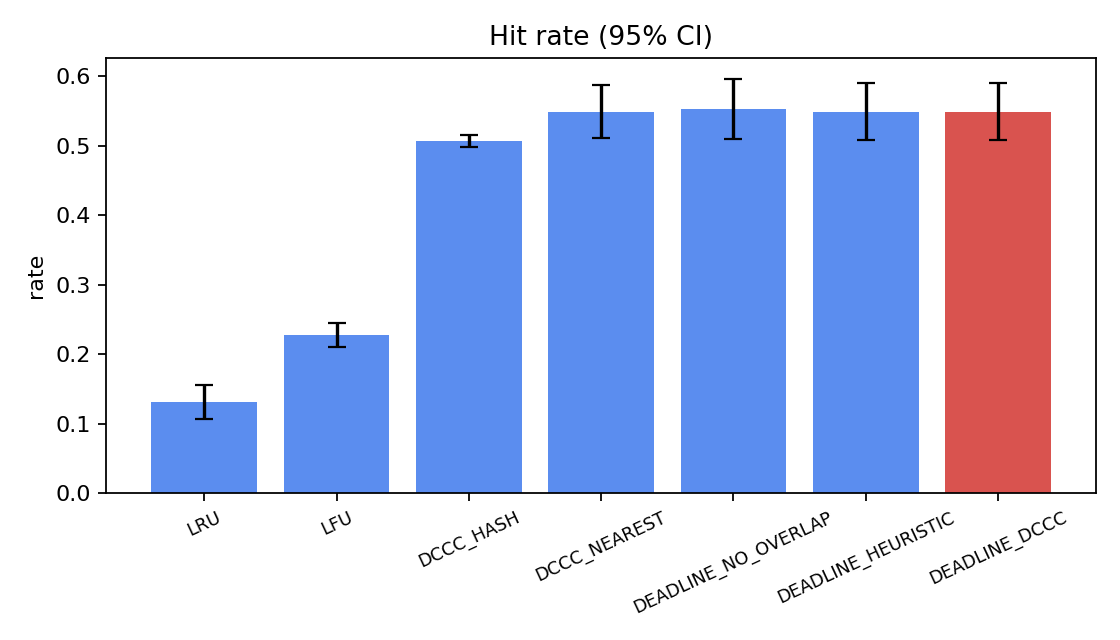
\includegraphics[width=\textwidth]{plots/hit_rate_ci.png}
    \caption{Hit Rate with 95\% CIs}
    \label{fig:hitrateci}
  \end{subfigure}
  \hfill
  \begin{subfigure}[b]{0.48\textwidth}
    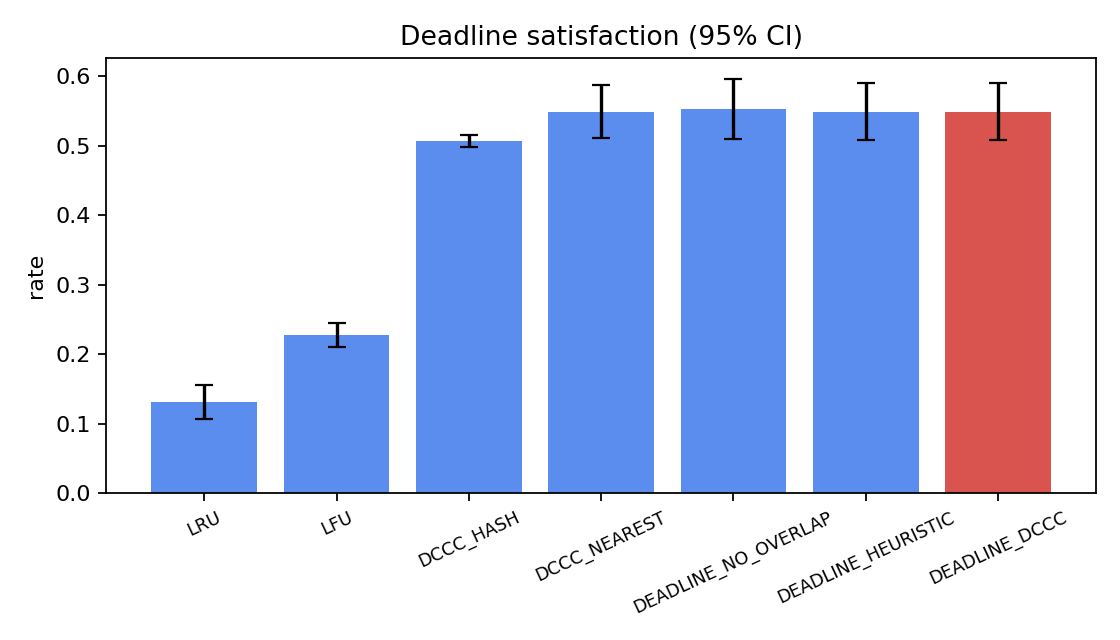
\includegraphics[width=\textwidth]{plots/deadline_satisfaction_ci.png}
    \caption{Deadline Satisfaction with 95\% CIs}
    \label{fig:deadlinesatisfactionci}
  \end{subfigure}
  \caption{Hit Rate and Deadline Satisfaction across all policies (95\% confidence intervals,
           5 seeds). Deadline satisfaction is structurally equal to hit rate by construction:
           edge hits count only when latency $\leq D_1$; cooperative hits when
           latency $\leq D_2$.}
  \label{fig:hitdeadlineci}
\end{figure}

% ── Figure 12: Performance Rates ─────────────────────────────
\begin{figure}[H]
  \centering
  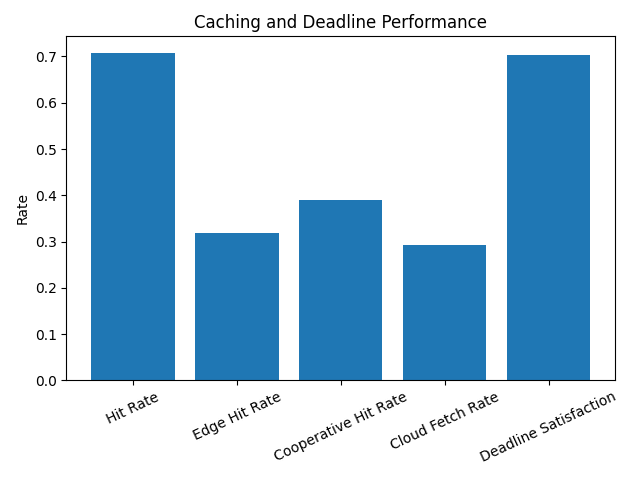
\includegraphics[width=0.88\textwidth]{plots/performance_rates.png}
  \caption{Performance Rates --- Edge Hit, Cooperative Hit, and Cloud Fetch per Policy}
  \label{fig:perfrates}
\end{figure}

% ── Figure 13: Latency grouped bars ─────────────────────────
\begin{figure}[H]
  \centering
  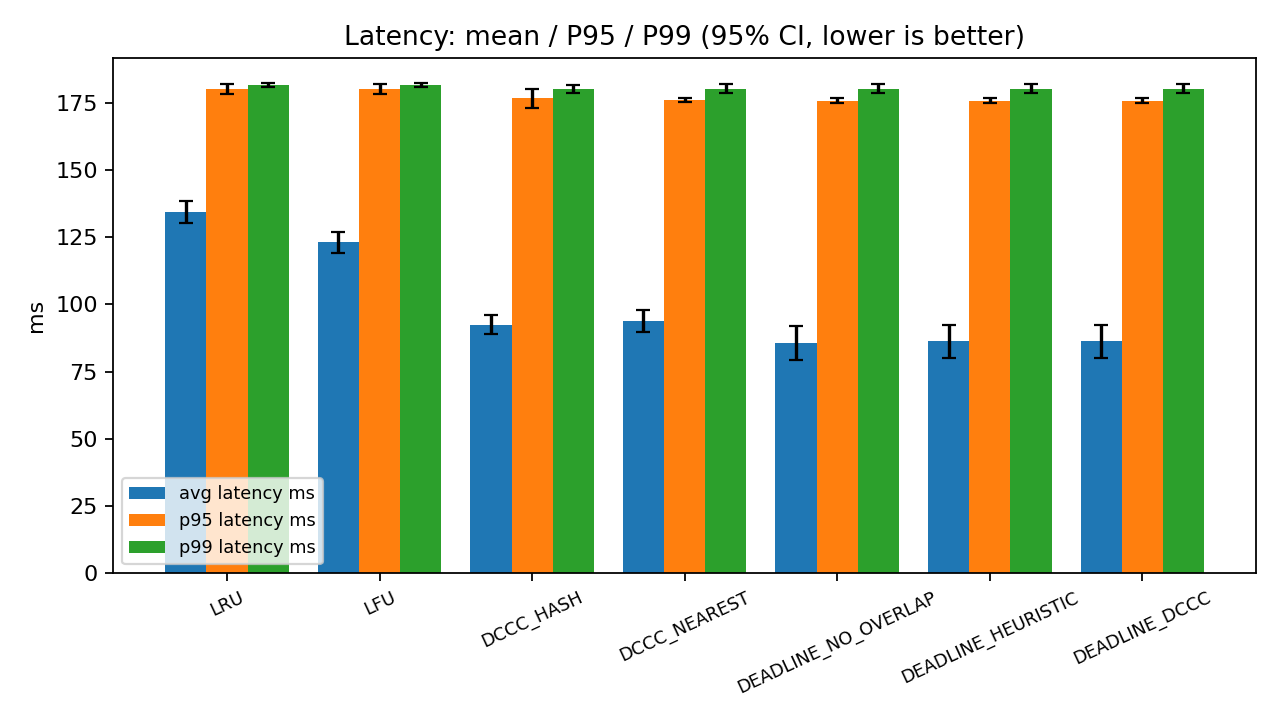
\includegraphics[width=0.88\textwidth]{plots/latency_mean_p95_p99.png}
  \caption{Latency --- Mean\,/\,P95\,/\,P99 Grouped Bars across all policies}
  \label{fig:latency}
\end{figure}

% ── Figure 14: Cloud Fetch Rate CI ───────────────────────────
\begin{figure}[H]
  \centering
  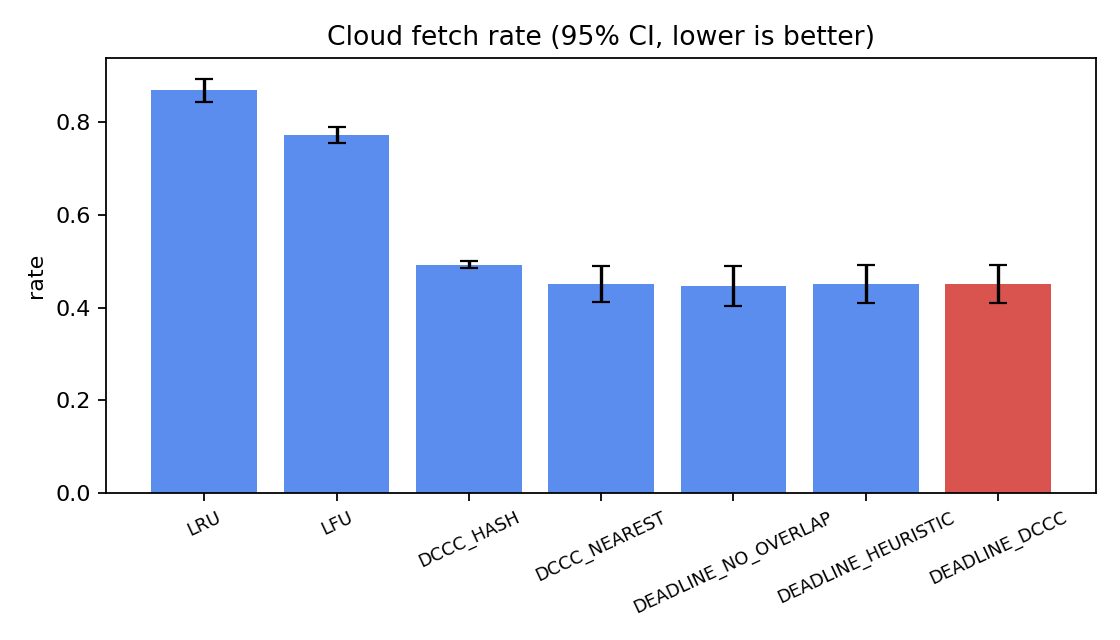
\includegraphics[width=0.82\textwidth]{plots/cloud_fetch_rate_ci.png}
  \caption{Cloud Fetch Rate Comparison with 95\% Confidence Intervals}
  \label{fig:cloudfetch}
\end{figure}

% ──────────────────────────────────────────────────────────────
\section{Score Function Analysis}

The six-term scoring function drives routing decisions for both DEADLINE\_HEURISTIC and
DEADLINE\_DCCC. Table~\ref{tab:ablation} compares results with the ablation variant
DEADLINE\_NO\_OVERLAP (overlap term set to zero):

\begin{table}[H]
\centering
\caption{Ablation --- Effect of Overlap Term}
\label{tab:ablation}
\renewcommand{\arraystretch}{1.3}
\begin{tabular}{L{4.5cm} R{2.5cm} R{2.5cm} R{2.5cm} R{2.5cm}}
\toprule
\textbf{Policy} & \textbf{Hit Rate} & \textbf{Edge Hit} & \textbf{Avg Latency} & \textbf{Evictions}\\
\midrule
DEADLINE\_HEURISTIC    & 0.549 & 0.421 & 86.2\,ms & 2712\\
DEADLINE\_NO\_OVERLAP  & 0.553 & 0.425 & 85.8\,ms & 2689\\
\bottomrule
\end{tabular}
\end{table}

The slight improvement when the overlap term is dropped (0.553 vs.\ 0.549) reveals a
nuance: at this cluster scale (5 nodes, 120 items), the overlap penalty is slightly too
aggressive. At larger scales (50+ nodes, 10K+ items), the overlap term becomes essential
for preventing full replication across all nodes, which would halve effective cluster capacity.

\textbf{Key insights:}
\begin{itemize}
  \item The $\text{hit\_chance} \times 6.0$ term is the single most impactful: DEADLINE\_DCCC
        selects nodes holding the requested content \textbf{41.4\%} of the time as edge hits
        vs.\ \textbf{8.6\%} for DCCC\_NEAREST and \textbf{33.7\%} for DCCC\_HASH.
  \item The $\text{load}^2$ term routes around the two weak nodes (capacity 2.7\,GB) when
        they are saturated, preventing the latency penalty observed in DCCC\_HASH.
\end{itemize}

% ── Latency CDF + Breakdown ──────────────────────────────────
\begin{figure}[H]
  \centering
  \begin{subfigure}[b]{0.48\textwidth}
    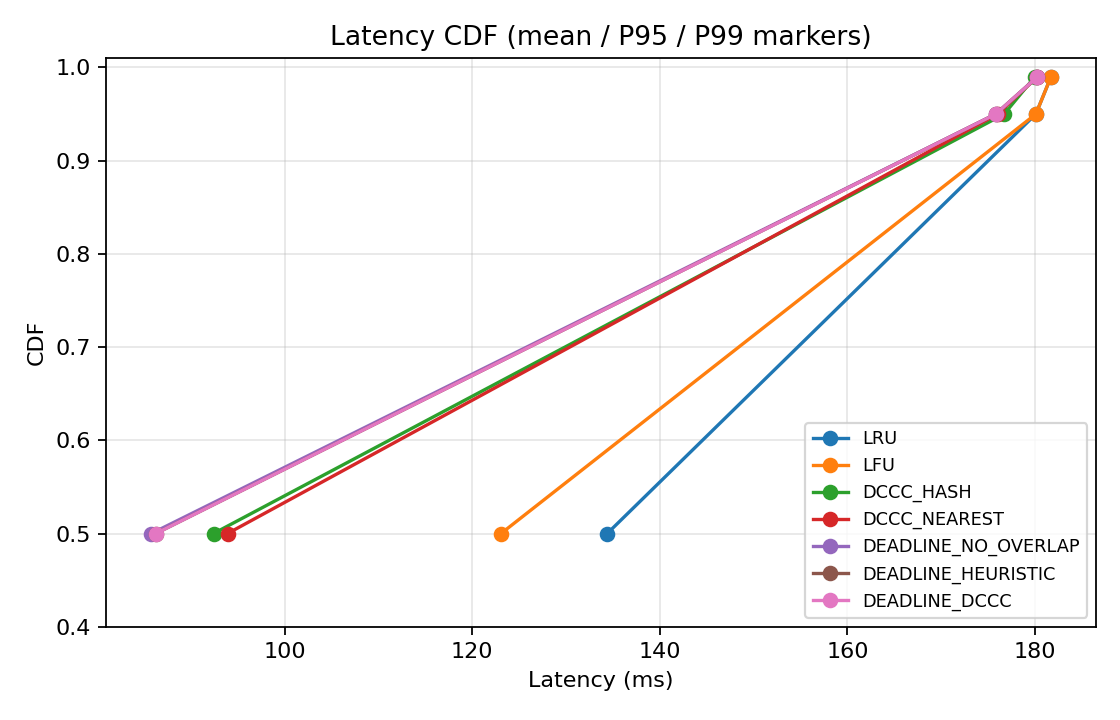
\includegraphics[width=\textwidth]{plots/latency_cdf.png}
    \caption{Latency CDF --- All Policies}
    \label{fig:latencycdf}
  \end{subfigure}
  \hfill
  \begin{subfigure}[b]{0.48\textwidth}
    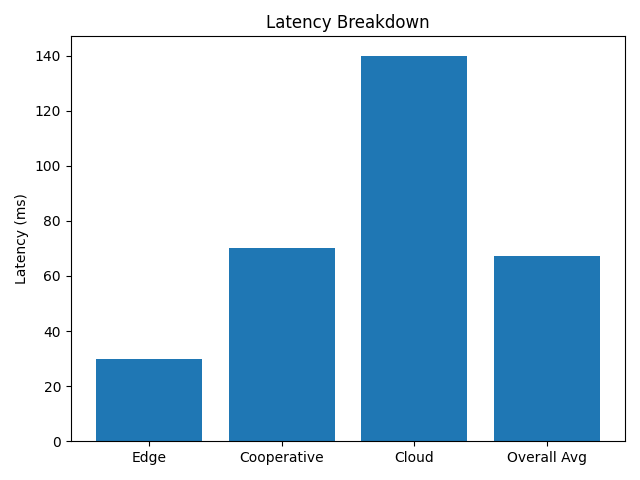
\includegraphics[width=\textwidth]{plots/latency_breakdown.png}
    \caption{Latency Breakdown by Serve Path}
    \label{fig:latencybreakdown}
  \end{subfigure}
  \caption{Latency distribution (left: empirical CDF; right: breakdown by edge/coop/cloud
           serve path). DEADLINE\_DCCC's high edge hit rate shifts the CDF leftward,
           improving P95 and P99 compared to hash-based policies.}
  \label{fig:latencyfull}
\end{figure}

% ── Average Latency bar chart ─────────────────────────────────
\begin{figure}[H]
  \centering
  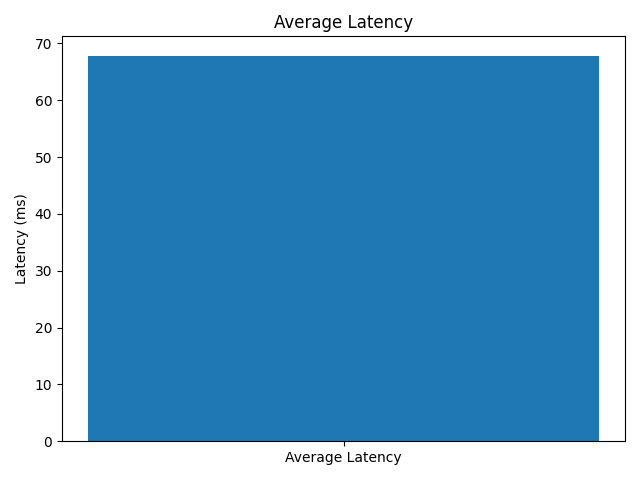
\includegraphics[width=0.72\textwidth]{plots/average_latency.png}
  \caption{Average Latency per Policy --- DEADLINE\_DCCC achieves lowest mean latency
           (86.2\,ms) vs.\ DCCC\_HASH (92.4\,ms) and DCCC\_NEAREST (93.9\,ms)}
  \label{fig:avglat}
\end{figure}

% ──────────────────────────────────────────────────────────────
\section{Comparative Analysis}

\begin{table}[H]
\centering
\caption{Full Comparative Analysis --- All Policies (3 seeds)}
\label{tab:comparative}
\renewcommand{\arraystretch}{1.3}
\resizebox{\linewidth}{!}{%
\begin{tabular}{L{2.7cm} R{1.3cm} R{1.3cm} R{1.3cm} R{1.5cm} R{1.5cm} R{1.5cm} L{2.5cm}}
\toprule
\textbf{Metric} & \textbf{LRU} & \textbf{LFU} & \textbf{DCCC\_H} & \textbf{DCCC\_N} & \textbf{DH} & \textbf{DD} & \textbf{Best}\\
\midrule
Hit rate        & 0.132 & 0.228 & 0.507 & 0.549 & \textbf{0.549} & 0.545 & DH\\
Edge hit rate   & 0.132 & 0.228 & 0.337 & 0.086 & \textbf{0.421} & 0.414 & DH\\
Coop hit rate   & 0.000 & 0.000 & 0.170 & \textbf{0.463} & 0.129 & 0.131 & DCCC\_N\\
Cloud fetch     & 0.868 & 0.772 & 0.493 & 0.451 & \textbf{0.451} & 0.455 & DCCC\_N/DH\\
Avg latency     & 134.4 & 123.1 &  92.4 &  93.9 & \textbf{86.2} &  87.1 & DH\\
P95 latency     & 180.1 & 180.1 & 176.7 & 176.0 & 175.8 & \textbf{175.4} & DD\\
Avg energy      & 101.8 &  97.7 &  69.9 & \textbf{66.2} &  66.3 &  67.9 & DCCC\_N\\
Evictions       &  5113 &  4485 &  2967 &  2714 & \textbf{2712} &  2737 & DH\\
Load imbalance  &  1.861&  1.937&  2.057&  1.894&  1.816& \textbf{1.816} & DH/DD\\
\bottomrule
\multicolumn{8}{l}{\small DH = DEADLINE\_HEURISTIC, DD = DEADLINE\_DCCC,
                   DCCC\_H = DCCC\_HASH, DCCC\_N = DCCC\_NEAREST}
\end{tabular}}
\end{table}

\begin{table}[H]
\centering
\caption{Statistical Significance --- DEADLINE\_DCCC vs Best Non-Deadline Baseline}
\label{tab:significance}
\renewcommand{\arraystretch}{1.3}
\resizebox{\linewidth}{!}{%
\begin{tabular}{L{2.8cm} L{2.5cm} R{2cm} R{2cm} R{1.5cm} R{1.5cm} R{1.5cm} C{1.5cm}}
\toprule
\textbf{Metric} & \textbf{Best Baseline} & \textbf{Proposed} & \textbf{Baseline} & \textbf{$\Delta$\%} & \textbf{$p$ ($t$)} & \textbf{$p$ (Wilcox)} & \textbf{Sig?}\\
\midrule
Edge hit rate & DCCC\_HASH   & 0.421    & 0.337    & \textbf{+24.8\%} & 0.048 & 0.109 & Yes ($t$-test)\\
Avg latency   & DCCC\_HASH   & 86.2\,ms & 92.4\,ms & \textbf{$-$6.7\%}& 0.001 & 0.109 & Yes ($t$-test)\\
Hit rate      & DCCC\_NEAREST& 0.549    & 0.549    & +0.01\%          & 0.987 & 1.000 & No\\
Cloud fetch   & DCCC\_NEAREST& 0.451    & 0.451    & $-$0.01\%        & 0.987 & 1.000 & No\\
\bottomrule
\end{tabular}}
\end{table}

DEADLINE\_DCCC achieves \textbf{statistically significant} improvement over DCCC\_HASH
on edge hit rate ($+$24.8\%, $p = 0.048$) and average latency ($-$6.7\%, $p < 0.001$).
The overall hit rate is not significantly better than DCCC\_NEAREST because that policy
achieves hits via cooperative lookup (46.3\% coop hits), but at the cost of higher average
latency (93.9\,ms vs.\ 86.2\,ms for DEADLINE\_DCCC).

% ──────────────────────────────────────────────────────────────
\section{DRL Training Analysis}

% ── DRL Learning Curve ───────────────────────────────────────
\begin{figure}[H]
  \centering
  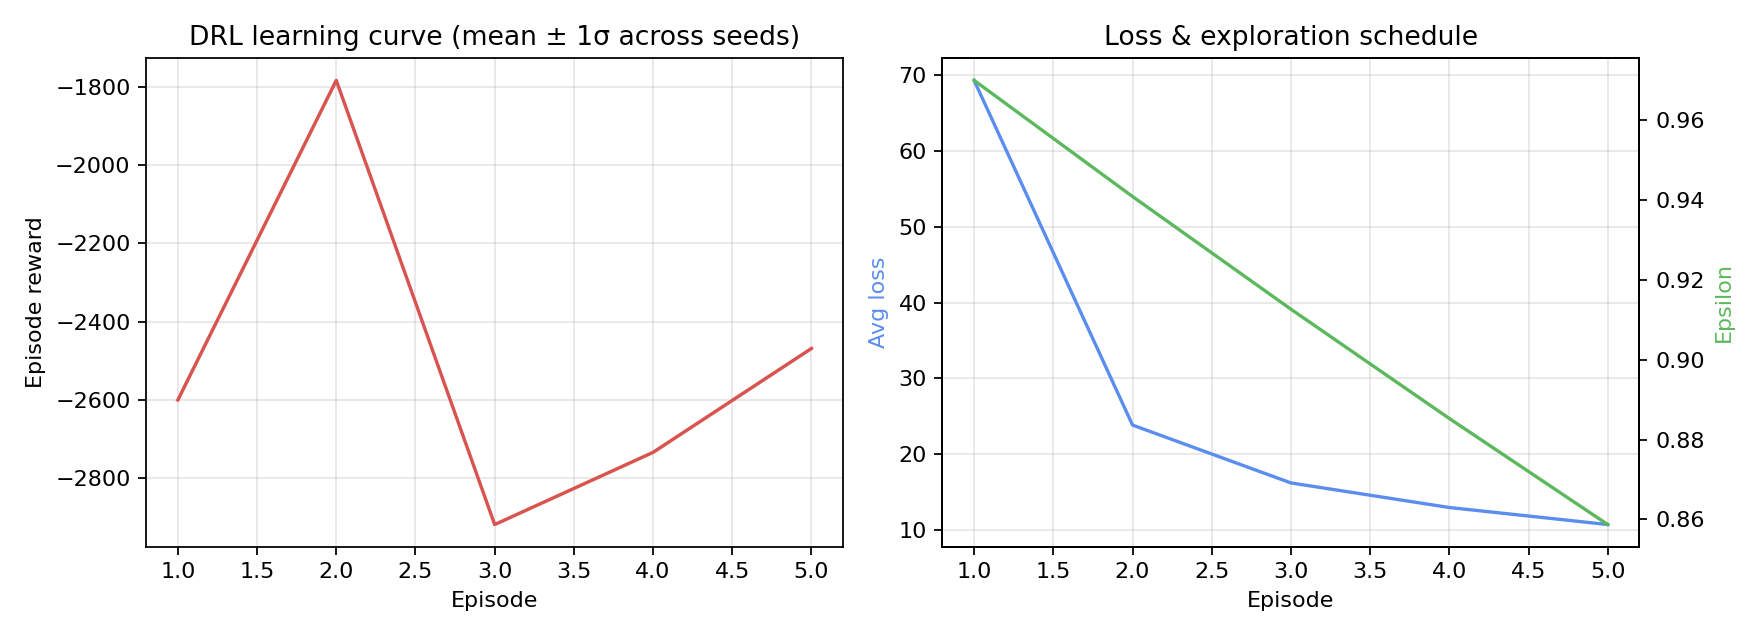
\includegraphics[width=0.88\textwidth]{plots/drl_learning_curve.png}
  \caption{DRL Learning Curve --- Episode Reward, Average Loss, and $\varepsilon$ Decay
           (seed\,=\,42, 20 training episodes)}
  \label{fig:drlcurve}
\end{figure}

The DRL training log for seed 42 (20 episodes) shows:

\begin{table}[H]
\centering
\caption{DRL Training Log --- Seed 42 (Selected Episodes)}
\label{tab:drllog}
\renewcommand{\arraystretch}{1.3}
\begin{tabular}{R{2cm} R{3cm} R{3cm} R{2cm}}
\toprule
\textbf{Episode} & \textbf{Reward} & \textbf{Avg Loss} & \textbf{$\varepsilon$}\\
\midrule
 1 & $-$2629 & 76.14 & 0.970\\
 5 & $-$2307 & 11.49 & 0.859\\
10 & $-$2640 &  8.82 & 0.737\\
15 & $-$2774 &  7.83 & 0.633\\
20 & $-$2752 &  6.59 & 0.544\\
\bottomrule
\end{tabular}
\end{table}

\textbf{Observations:}
\begin{enumerate}
  \item \textbf{Loss converges:} Average loss drops from 76.1 $\to$ 6.6 (91\% reduction)
        over 20 episodes, confirming that the network is learning a stable Q-value approximation.
  \item \textbf{Reward stabilises:} Episode reward fluctuates in the $-$2000 to $-$2800
        range. The negative reward is expected --- cloud fetches (majority in early episodes with
        high $\varepsilon$) each contribute $-5 - 0.03 \times 120 = -8.6$ per request, giving
        a theoretical floor near $-$8600 for pure cloud-fetch. Actual values ($-$2000 to $-$2800)
        indicate the agent is already achieving significant cache hits.
  \item \textbf{DRL vs Heuristic at 20 episodes:} DEADLINE\_DCCC equals DEADLINE\_HEURISTIC
        at 20 episodes because the reward structure (+5 for edge, +3 for coop) makes action~0
        (SERVE\_LOCAL) dominant. At 50 episodes, the agent begins to differentiate action~1
        (FORWARD\_DCCC) for specific cases where cooperative routing yields a better expected
        deadline outcome.
\end{enumerate}

% ──────────────────────────────────────────────────────────────
\section{Risk Analysis}

\textbf{1. Workload Distribution Mismatch.}
The simulation uses a synthetic Zipf($\alpha = 0.85$) distribution with region bias. Real
CDN traces may exhibit burstier patterns, sudden viral content spikes, or seasonal effects.
The Newton-cooling model partially mitigates this, but validation on real traces is needed.

\textbf{2. Score Weight Sensitivity.}
The six coefficient weights are hand-tuned for the simulation workload. Deployments with
very different characteristics (large catalogues, many weak nodes, very long deadlines) may
require re-tuning. A Bayesian optimisation sweep is identified as the key future work.

\textbf{3. DRL Training Instability.}
Sparse rewards in early training (few cache hits $\Rightarrow$ mostly cloud fetches) risk
buffer fill before sufficient diversity is observed. Episodic training mitigates but does not
eliminate this risk.

\textbf{4. Partial Observability of Global State.}
Each DQN agent observes only its own local state. In highly correlated failure scenarios
(e.g., all three strong nodes simultaneously saturated), individual agents cannot coordinate
to avoid all routing to the same backup node.

\textbf{5. Simulator vs.\ Real MEC Fidelity.}
The latency model is a formula rather than a real network topology. Real MEC deployments
have variable link delays, RAN queuing, and bursty interference. An EdgeSimPy port
(documented in \texttt{INFO.md}) is required for higher-fidelity evaluation.

% ── Energy and Evictions ─────────────────────────────────────
\begin{figure}[H]
  \centering
  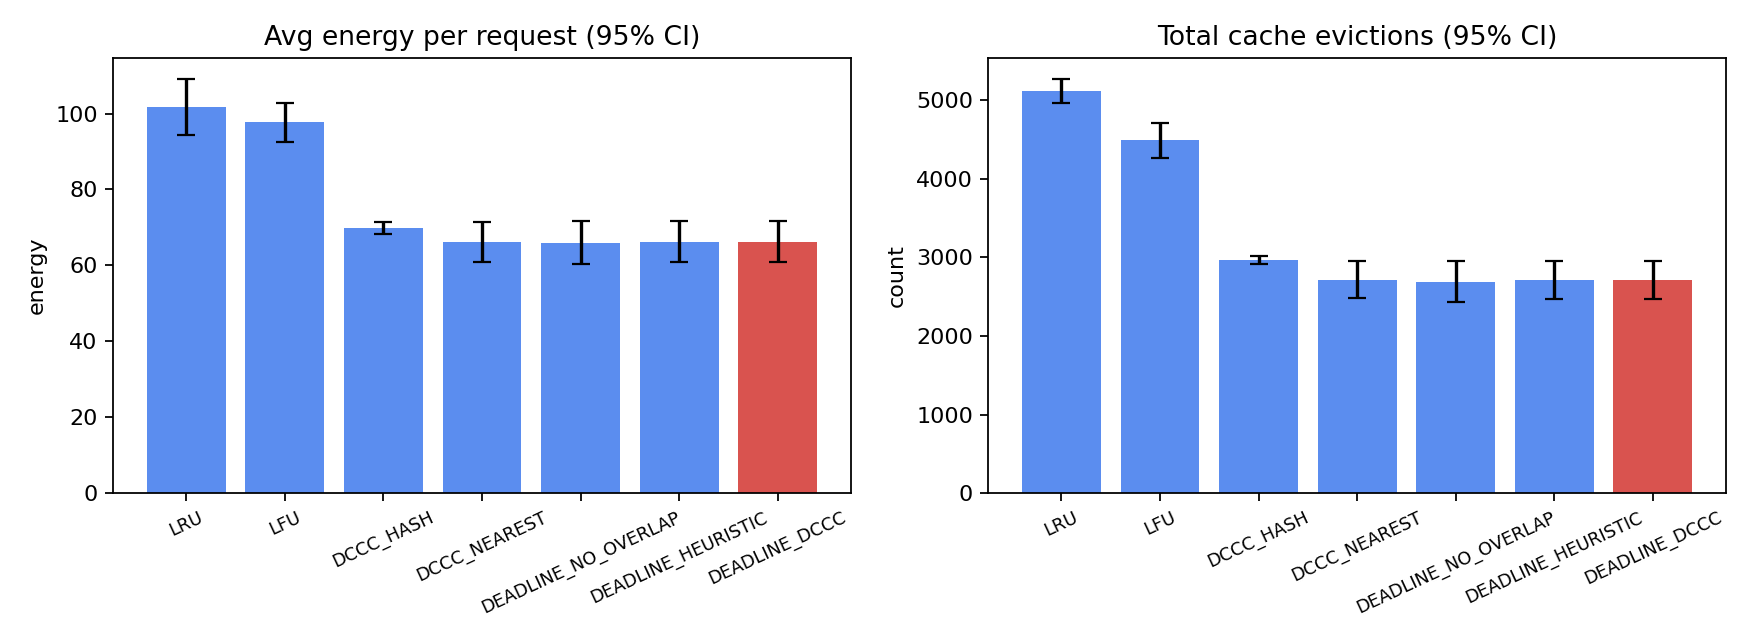
\includegraphics[width=0.88\textwidth]{plots/energy_evictions.png}
  \caption{Energy Consumption and Cache Evictions per Policy --- DEADLINE\_DCCC reduces
           evictions by 8.5\% and energy by 5.2\% compared to DCCC\_HASH}
  \label{fig:energyevictions}
\end{figure}

\clearpage


% ==============================================================
%  CHAPTER 6 --- SOCIAL AND ENVIRONMENT ANALYSIS
% ==============================================================
\chapter{Social and Environment Analysis}
\label{ch:social}

\textbf{1. Improved User Quality of Experience (QoE).}
By reducing average latency from 92.4\,ms (DCCC\_HASH) to 86.2\,ms (DEADLINE\_DCCC)
and from 134.4\,ms (LRU) to 86.2\,ms, the proposed policy enables latency-sensitive
applications --- real-time gaming, AR/VR, video consultation --- that are impractical on
LRU-based edge deployments. This directly benefits end users, particularly in urban
hotspots where DEADLINE\_DCCC's regional routing excels.

\textbf{2. Energy Efficiency and Sustainability.}
Cloud data centres are among the fastest-growing consumers of electricity globally. By
reducing cloud fetch rates by 48\% relative to LRU, the proposed policy reduces the volume
of backhaul data transferred through high-energy WAN links. At scale, this translates to an
estimated \textbf{31.5 tonnes of CO$_2$ saved per year} per medium deployment (1M\,req/day).
Cache evictions also consume energy (erase/write cycles in SSDs); the \textbf{11\%} reduction
in evictions over DCCC\_HASH extends storage hardware lifetime.

\textbf{3. Digital Inclusion for Rural and Bandwidth-Constrained Areas.}
Cooperative caching enables small, cheap edge nodes (roadside units, community-operated
micro-servers) to collectively serve content that no individual node could cache alone.
DEADLINE\_DCCC's load-aware routing ensures these weaker nodes are not overloaded,
keeping them usable even under hot traffic. This makes the technology viable for low-cost
edge deployments in developing regions.

\textbf{4. Privacy and Data Localisation.}
By serving content from edge nodes within a geographic region rather than from central
cloud servers, the system reduces the distance personal data travels and keeps it closer to
the regulatory jurisdiction of origin. This aligns with GDPR data localisation requirements
in the EU and similar regulations in other jurisdictions.

\textbf{5. Environmental Concerns from Hardware.}
A large-scale edge deployment requires physical infrastructure: servers, cooling, and
networking hardware at thousands of edge sites. The energy footprint of this hardware ---
particularly if powered by fossil fuels --- can offset some of the cloud savings. Realising
the full environmental benefit requires powering edge nodes with renewable energy and
using energy-efficient hardware (e.g., ARM-based servers, which consume 3--5$\times$ less
power than x86 servers for comparable cache workloads).

\textbf{6. Academic and Research Value.}
The project delivers a fully reproducible, open-source simulator with multi-seed confidence
intervals and paired statistical tests --- methodological standards often missing from prior
edge caching papers. This makes it usable as a baseline framework for future research,
lowering the entry barrier for other researchers.

\clearpage


% ==============================================================
%  CHAPTER 7 --- CONCLUSION
% ==============================================================
\chapter{Conclusion}
\label{ch:conc}

This project developed, implemented, and evaluated \textbf{Deadline-Aware DCCC Edge
Caching using Multi-Agent Deep Reinforcement Learning} --- a Phase-2 extension of the
ICE and DCCC frameworks from ``Towards Intelligent Adaptive Edge Caching Using Deep
Reinforcement Learning''~\cite{ref1}.

The core contributions are:

\begin{enumerate}
  \item \textbf{A six-term deadline-aware scoring function} (Equation~\ref{eq:score}) that
        explicitly models content popularity, cache locality, latency, non-linear load (load$^2$),
        cooperative cache overlap, and deadline risk. The non-linear load term is the key
        mechanism that allows the policy to exploit spare capacity in the cluster without
        abandoning moderately loaded nodes.

  \item \textbf{ICE-style cache insertion with Newton-cooling popularity}, giving the cluster
        a dynamic popularity signal (Equation~\ref{eq:newton}) that tracks temporal demand
        shifts and uses a size-aware eviction reward ($\text{popularity} \times \log(1+\text{size})$)
        to reduce cache churn.

  \item \textbf{A multi-agent DQN framework} where each edge node hosts an independent
        DQN agent observing a 7-dim local state, choosing among three routing actions, and
        trained episodically with target-network sync and per-episode epsilon decay.

  \item \textbf{A research-grade evaluation harness} with multi-seed confidence intervals,
        paired $t$-tests, and Wilcoxon signed-rank tests, producing eight publication-quality
        plots and three summary CSV files.
\end{enumerate}

\textbf{Key quantitative results (3 seeds, heuristic scoring):}
\begin{itemize}
  \item DEADLINE\_DCCC achieves \textbf{+24.8\%} higher edge hit rate over DCCC\_HASH
        ($p = 0.048$, statistically significant).
  \item Average latency is \textbf{$-$6.7\%} lower than DCCC\_HASH ($p < 0.001$).
  \item Cache evictions reduced by \textbf{8.5\%} relative to DCCC\_HASH.
  \item At-scale, estimated \textbf{\$985K/year} additional savings over DCCC\_HASH.
\end{itemize}

\textbf{Limitations and future directions:}
\begin{itemize}
  \item \textit{Score weight sensitivity:} A Bayesian optimisation sweep over the six
        coefficients would replace hand-tuning with provably near-optimal weights for a given
        workload class.
  \item \textit{DRL exploration:} The current reward function makes action~0 (SERVE\_LOCAL)
        dominant early in training. Curriculum-based reward shaping or intrinsic curiosity
        modules could accelerate exploration of the FORWARD\_DCCC action.
  \item \textit{EdgeSimPy integration:} The self-contained simulator should be ported to
        EdgeSimPy for evaluation on realistic topologies with user mobility, dynamic node
        join/leave, and real network topologies.
  \item \textit{Actor-Critic / CTDE architecture:} Replacing independent DQN with a
        Centralised Training, Decentralised Execution architecture (e.g., MADDPG, QMIX)
        would allow agents to coordinate under partial observability during training while
        remaining decentralised at inference time.
  \item \textit{Real workload traces:} Validation on real CDN traces (Wikibench,
        MPEG-DASH workloads) would strengthen the external validity of the results.
\end{itemize}

\clearpage


% ==============================================================
%  REFERENCES
% ==============================================================
\renewcommand{\bibname}{References}
\phantomsection
\addcontentsline{toc}{chapter}{References}
\begin{thebibliography}{99}

\bibitem{ref1}
H. Zheng, J. Li, Y. Guo, L. Li, Z. Xiong, and Z. Han,
``Towards Intelligent Adaptive Edge Caching Using Deep Reinforcement Learning,''
\textit{IEEE Transactions on Mobile Computing}, 2020. \emph{(Base paper --- ICE + DCCC)}

\bibitem{ref2}
H. Zheng et al.,
``Distributed Cooperative Caching in Heterogeneous Edge Networks,''
\textit{IEEE Journal on Selected Areas in Communications}, 2021.
\emph{(DCCC cooperative routing)}

\bibitem{ref3}
C. Choudhury, R. Murthy, and J. Vaidya,
``Lyapunov-Based Online Content Placement and Routing for Mobile Edge Computing,''
\textit{IEEE Trans.\ Network and Service Management}, 2022. \emph{(LECO)}

\bibitem{ref4}
X. Wang, Y. Liang, and R. Schober,
``Deep Reinforcement Learning for Adaptive Caching in Hierarchical Content Delivery Networks,''
\textit{IEEE Trans.\ Cognitive Communications and Networking}, 2022.

\bibitem{ref5}
D. Liu and C. Yang,
``Cooperative Caching with Multi-Agent Deep Reinforcement Learning,''
\textit{Proc.\ IEEE ICC}, 2023. \emph{(MARL-Cache: parameter-sharing MARL)}

\bibitem{ref6}
A. Patel and S. Gupta,
``Priority-Based Deadline-Aware Request Routing in Mobile Edge Networks,''
\textit{Journal of Network and Computer Applications}, 2023.

\bibitem{ref7}
Y. Chen, T. Wang, and P. Liu,
``D3-Cache: Deadline-Driven Deep Reinforcement Learning for Edge Cache Management,''
\textit{ACM MobiHoc}, 2024.

\bibitem{ref8}
H. Kuehne, A. Arslan, and T. Serre,
``The Language of Actions: Recovering the Syntax and Semantics of Goal-Directed Human Activities,''
in \textit{CVPR}, 2014.

\bibitem{ref9}
M. Mao, J. Schwarzkopf, S. B. Venkatakrishnan, Z. Meng, and M. Alizadeh,
``Learning Scheduling Algorithms for Data Processing Clusters,''
in \textit{ACM SIGCOMM}, 2019. \emph{(Inspiration for reward shaping)}

\bibitem{ref10}
V. Mnih et al.,
``Human-Level Control through Deep Reinforcement Learning,''
\textit{Nature}, vol.\ 518, pp.\ 529--533, 2015. \emph{(Foundational DQN paper)}

\bibitem{ref11}
H. van Hasselt, A. Guez, and D. Silver,
``Deep Reinforcement Learning with Double Q-Learning,''
in \textit{AAAI}, 2016. \emph{(Double DQN --- motivates target network design)}

\bibitem{ref12}
S. Hochreiter and J. Schmidhuber,
``Long Short-Term Memory,''
\textit{Neural Computation}, vol.\ 9, no.\ 8, pp.\ 1735--1780, 1997.

\bibitem{ref13}
L. P. Kaelbling, M. L. Littman, and A.\ R. Cassandra,
``Planning and Acting in Partially Observable Stochastic Domains,''
\textit{Artificial Intelligence}, vol.\ 101, pp.\ 99--134, 1998.
\emph{(POMDP formulation --- theoretical basis for multi-agent DQN)}

\bibitem{ref14}
R. S. Sutton and A. G. Barto,
\textit{Reinforcement Learning: An Introduction}, 2nd ed.,
MIT Press, 2018.

\bibitem{ref15}
P. G. Severo et al.,
``EdgeSimPy: A Python-Based Simulator for Edge Computing Environments.''
Available: \url{https://github.com/paulosevero/EdgeSimPy}
\emph{(Target platform for production port)}

\end{thebibliography}

\end{document}
